\chapter{Rings and Ideals}

\section*{Rings and Ring Homomorphisms}
\addcontentsline{toc}{section}{Rings and Ring Homomorphisms}

Let $R$ be a commutative ring with identity.

\begin{fact}
    $R = 0$ if and only if $1_R = 0_R$.
\end{fact}

\begin{fact}
    \begin{enumerate}
        \item $1_R$ and $0_R$ are both unique.
        \item For any $r \in R$, $-r$ is unique.
        \item If $r \in R$ is a unit, then there exists a unique $r^{-1} \in R$ such that $rr^{-1} = 1_R = r^{-1}r$.
    \end{enumerate}
\end{fact}

\begin{definition}
    A \emph{(unital) homomorphism of commutative rings with identity} is a function $\phi: R \to S$ with $R$ and $S$ commutative rings with identity, such that for all $r,r' \in R$,
    \begin{enumerate}
        \item $\phi(r+r') = \phi(r) + \phi(r')$,
        \item $\phi(rr') = \phi(r) \phi(r')$,
        \item $\phi(1_R) = 1_S$.
    \end{enumerate}
    It is also known as ``ring homomorphism''.
\end{definition}

\begin{fact}
    Let $\phi: R \to S$ be a ring homomorphism.
    \begin{enumerate}
        \item $\phi(0_R) = 0_S$.
        \item $\phi(-r) = -\phi(r)$ for any $r \in R$.
        \item $\phi(r-s) = \phi(r) - \phi(s)$ for any $r,s \in R$.
        \item $\phi(\sum_{i=1}^mr_is_i) = \sum_{i=1}^m\phi(r_i)\phi(s_i)$ for any $r_1,\cdots,r_m,s_1,\cdots,s_m \in R$.
        \item If $r$ is a unit in $R$, then $\phi(r)$ is a unit in $S$ and $\phi(r)^{-1} = \phi(r^{-1})$.
        \item A composition of ring homomorphisms is a ring homomorphism.
    \end{enumerate}
\end{fact}

\begin{definition}
    A \emph{subring} of $R$ is a subset $S \subseteq R$ such that $S$ is a commutative ring with identity under the operations for $R$ and such that $1_S = 1_R$, i.e., $1_R \in S$.
\end{definition}

\begin{fact}[Subring test]
    A subset $S \subseteq R$ is a subring if and only if it is closed under $+,\cdot,-$ and $1_R \in S$.
\end{fact}

\begin{example}
    Subring test: need $\emptyset \neq S \subseteq R$, $S$ is closed under $+,\cdot,-$ and $1_R \in S$. \par
    If $S$ is not closed under $-$, then fail. Let $\bbN_0 = \{0,1,2,\cdots\} \subseteq \bbZ$ not a subring. \par
    If $1_R \not \in S$, then fail. Let $R = \bbF_3 \times \bbF_3 \supseteq \{(a,a) \mid a \in \bbF_3\} =: S$. Then $S$ is a subring of $R$. Although $S_1 := \{(a,0) \mid a \in \bbF_3\} \cong \bbF_3 \cong \{(0,a) \mid a \in \bbF_3\} =: S_2$ are rings but not subrings of $R$ since $1_R = (1,1) \not \in S_1$ and $1_R = (1,1) \not \in S_2$. 
\end{example}

\begin{fact}
    If $S \subseteq R$ is a subring, then the inclusion map $\varepsilon: S \to R$ given by $\varepsilon(s) = s$ is a ring homomorphism.
\end{fact}

\section*{Ideals and Generators}
\addcontentsline{toc}{section}{Ideals and Generators}

\begin{definition}
    An \emph{ideal} of $R$ is a non-empty subset $\ffa \subseteq R$, an additive subgroup such that for any $r \in R$ and any $a \in \ffa$, $ra \in \ffa$, i.e., closed under scalar multiplication. \par
    An ideal $\ffa \leq R$ is \emph{prime} if $\ffa \neq R$ and for any $a,b \in R$, if $a,b \not \in \ffa$, then $ab \not \in \ffa$, i.e., if $ab \in \ffa$, then $a \in \ffa$ or $b \in \ffa$. \par
    An ideal $\ffa \leq R$ is \emph{maximal} if $\ffa \neq R$ and for any ideal $\ffb \leq R$, if $\ffa \subseteq \ffb \subseteq R$, then either $\ffa = \ffb$ or $\ffb = R$.
\end{definition}

\begin{fact}[Ideal test]
    If $\ffa \neq \emptyset$ and $\ffa$ is closed under scalar multiplication $\cdot$, then for any $a \in \ffa$, $-a = (-1_R)a \in \ffa$, also, since $\ffa$ is closed under $+$, it is automatically closed under $-$. \par
    Thus, A subset $\ffa \subseteq R$ is an ideal if and only if $\ffa \neq \emptyset$ and $\ffa$ is closed under $+$ and scalar multiplication $\cdot$. 
\end{fact}

\begin{example}
    \begin{enumerate}
        \item 
            Let $R = \bbZ$, then ideals of $R$ are of the form $n\bbZ = \{nm \mid m \in \bbZ\}$, where $n \in \bbZ$. \par 
            $n\bbZ$ is prime if and only if $n = 0$ or $\abs n$ is prime. \par
            $n\bbZ$ is maximal if and only if $\abs n$ is prime.
        \item 
            If $I_\lambda \leq R$ for any $\lambda \in \Lambda$, then $\bigcap_{\lambda \in \Lambda} I_\lambda \leq R$.
        \item 
            If $r_1,\cdots,r_m \in R$, then 
            \begin{align*}
                \langle r_1,\cdots,r_m \rangle &= \langle r_1,\cdots,r_m \rangle R = (r_1,\cdots,r_m) = (r_1,\cdots,r_m)R = \bigcap_{r_1,\cdots,r_m \in I \leq R} I \\
                                               &= \left\{\sum_{i=1}^m a_ir_i \mathrel{\bigg |} a_i \in R, \fa i = 1,\cdots,m\right\} \leq R. 
            \end{align*}
            In particular, for any $r \in R$, $\langle r \rangle = \langle r \rangle R = (r) = (r)R = rR = Rr = \{ar \mid a \in R\} = \bigcap_{r \in I \leq R}I$.
        \item 
            If $A \subseteq R$, then $\langle A \rangle = \bigcap_{A \subseteq I \leq R}I$ and 
            \[\langle A \rangle = RAR = AR = RA = \left\{\sum_{a \in A}^{\text{finite}} r_a a \mathrel{\bigg |} r_a \in R, \fa a \in \ffa\right\}\].
    \end{enumerate}
\end{example}

\begin{fact}
    For any $r_1,\cdots,r_m \in R$, $\langle r_1,\cdots,r_m \rangle$ is the smallest ideal of $R$ containing $r_1,\cdots,r_m$, i.e., for any $\ffa \leq R$, $r_1,\cdots,r_m \in \ffa$ if and only if $\langle r_1,\cdots,r_m \rangle \subseteq \ffa$. Similarly, $A \subseteq \ffa$ if and only if $\langle A \rangle \subseteq \ffa$, e.g., if $A \leq R$, then $A = \langle A \rangle$.
\end{fact}

\begin{construction}
    Let $\ffa \leq R$. For any $r \in R$, $r+\ffa = \{r + a \mid a \in \ffa\} = \overbar r$. Let 
    \[R/\ffa := \{r + \ffa \mid r \in R\}.\] 
    \par Then $R/\ffa$ is a commutative ring with identity with $\overbar r \pm \overbar s = \overbar {r \pm s}$, $\overbar r \overbar s = \overbar{rs}$, $0_{R/\ffa} = \overbar {0_R}$ and $1_{R/\ffa} = \overbar {1_R}$. \par
    Let $\pi: R \to R/\ffa$ be given by $\pi(r) = \overbar r$. Then $\pi$ is a well-defined ring epimorphism. \par 
    (UMP) For any $\phi: R \to S$ ring homomorphism, if $\phi(\ffa) = 0$, then there exists a unique ring homomorphism $\overbar \phi: R/\ffa \to S$ making the following diagram commute. 
    \begin{center} 
        \begin{tikzcd}
            R \ar[rrr,"\phi"] \ar[ddd,swap,"\pi"] &[-30pt] & &[-10pt] S \\ [-20pt]
            &r \ar[r,mapsto] \ar[d,mapsto] & \phi(r) \\ 
            &\overbar{r} \ar[ru, mapsto] \\ [-5pt]
            R/\ffa \ar[rrruuu,dashed,swap,"\ex !\ \overbar{\phi}"]
        \end{tikzcd}
    \end{center}
    \par
    Note $\phi(\ffa) = 0$ if and only if $\ffa \subseteq \ker(\phi)$. In particular, if $\ffa = \langle A \rangle$, then $\ffa \subseteq \ker(\phi)$ if and only if $A \subseteq \ker(\phi)$.
\end{construction}

\begin{fact}
    Let $\ffa \leq R$. 
    \begin{enumerate}
        \item $\ffa$ is prime if and only if $R/\ffa$ is an integral domain.
        \item $\ffa$ is maximal if and only if $R/\ffa$ is a field.
        \item If $R$ is a field, then it is an integral domain. 
    \end{enumerate}
    So if $\ffa$ is maximal, then $\ffa$ is prime.
\end{fact}

\begin{fact}[Ideal correspondence for quotients]
    Let $\ffa \leq R$ and $\pi: R \to R/\ffa$ be the canonical ring epimorphism. 
    \begin{align*}
        \{\text{ideals }I \leq R/\ffa\} &\rightleftarrows \{\text{ideals }J \leq R \mid \ffa \subseteq J\} \\
        I &\mapsto \pi^{-1}(I) = \{r \in R \mid r + \ffa \in I\} \\
        J/\ffa &\mapsfrom J \\
    \{\text{ideals } I \leq R/\ffa\} &\rightleftarrows \{\text{ideals }J \leq R \mid \ffa \subseteq J\} \\
        \{\text{primes ideals of } R/\ffa\} &\rightleftarrows \{\text{prime ideals }\ffp \leq R \mid \ffa \subseteq \ffp\} \\
        \{\text{maximal ideals of } R/\ffa\} &\rightleftarrows \{\text{maximal ideals }\ffm \leq R \mid \ffa \subseteq \ffm\}.
    \end{align*}
    \par
    In both $R$ and $R/\ffa$, maximal ideals are a subset of prime ideals and prime ideals are a subset of ideals. \par
    Claim. $\frac{R/\ffa}{J/\ffa} \cong \frac{R}{J}$.
    \begin{center}
        \begin{tikzcd}
            R \ar[rr,"p"] \ar[ddd,swap,"\pi"] &[-30pt] & R/\ffa \ar[rr,"\tau"] & &[+15pt] \frac{R/\ffa}{J/\ffa} \\ [-25pt]
            & r \ar[r,mapsto] \ar[d,mapsto] & \overbar{r} \ar[r,mapsto] & \overbar{\overbar{r}} \\
            & \overbar{r} \ar[rru,mapsto] \\ [-18pt] 
            R/J \ar[rrrruuu,dashed,swap,"\ex !\ \overbar{\phi}"]
        \end{tikzcd}
    \end{center}
    \par 
    It is straightforward to show that $J = \ker(\tau \circ p)$. Then the first isomorphism theorem says the map $\overbar \phi$ is a ring isomorphism. 
\end{fact}

\begin{notation*}
    $\operatorname{Spec}(R) = \{\text{primes ideals of $R$}\}$, called the \emph{prime spectrum of} $R$. \\
    The variety determined by an ideal $\ffa \leq R$ is $\operatorname{V}(\ffa) = \{\ffp \in \operatorname{Spec}(R) \mid \ffp \supseteq \ffa\}$.
\end{notation*}

\begin{fact}
    Let $\phi: R \to S$ be a ring homomorphism. Then $\ker(\phi) \leq R$, $\im(\phi) \subseteq S$ is a subring and $\im(\phi) \cong R/\ker(\phi)$. \par 
    If $S$ is an integral domain, then so is $\im(\phi)$. Hence $\ker(\phi)$ is prime. \par
    More generally, for any $\ffb \leq S$, we have $\phi^{-1}(\ffb) = \{x \in R \mid \phi(x) \in \ffb\} \leq R$.
    \begin{center}
        \begin{tikzcd}
            R \ar[rr,"\phi"] \ar[ddd,swap,"p"] &[-35pt] & S \ar[rr,"\pi"] & &[+10pt] S/\ffq \\ [-25pt]
            & r \ar[r,mapsto] \ar[d,mapsto] & \phi(r) \ar[r,mapsto] & \overbar{\phi(r)} \\
            & \overbar{r} \ar[rru,mapsto] \\ [-20pt] 
            \frac{R}{\phi^{-1}(\ffq)} \ar[rrrruuu,dashed,swap,"\ex !\ \overbar{\pi \circ \phi}"]
        \end{tikzcd}
    \end{center}
    \par
    Let $\ffq \in \operatorname{Spec}(S)$. Then $S/\ffq$ is an integral domain. Also, since $R/\ker(\pi \circ \phi) \cong \im(\pi \circ \phi) \subseteq S/\ffq$, we have $R/\ker(\pi \circ \phi)$ is an integral domain and then $\ker(\pi \circ \phi)$ is prime. Observe $\phi^{-1}(\ffq) = \ker(\pi \circ \phi)$ is then prime, i.e., $\phi^{-1}(\ffq) \in \operatorname{Spec}(R)$. Thus, $\phi$ induces a well-defined map $\phi^*: \operatorname{Spec}(S) \to \operatorname{Spec}(R)$ given by $\phi^*(\ffq) = \phi^{-1}(\ffq)$.
    \end{fact}

\begin{example*}
    Let $\phi: \bbZ \to \bbQ$ be an inclusion map. Note $\ffq := (0)\bbQ \leq \bbQ$ is maximal, but $\phi^{-1}(\ffq) = \phi^{-1}(0) = \ker(\phi) = 0 \bbZ$, which is not maximal in $\bbZ$. So the map $\phi^*$ does not take maximal ideals to maximal ideals in general.
\end{example*}

\begin{fact}
    \begin{enumerate}
        \item 
            Let $R \neq 0$. Then $R$ has a maximal ideal $\ffm$ and so $R$ has a prime ideal. Moreover, for any $\ffa \lneq R$, there exists a maximal ideal $\ffm \supseteq \ffa$. In particular, $\operatorname{V}(\ffa) = \{\ffp \in \operatorname{Spec}(R) \mid \ffp \supseteq \ffa\} \neq \emptyset$. \par
            One generally proves the second statement first, then derives the first statement as the special case $\ffa = 0$. Next, we show how to derive the second statement from the first one.
        \item 
            Let $\ffa \lneq R$. Then $0 \neq R/\ffa$ is a commutative ring with identity. So $R/\ffa$ has a maximal ideal and by Fact 1.15, it is of the form $\ffm/\ffa$, where $\ffm$ is a maximal ideal of $R$ containing $\ffa$.
    \end{enumerate}
\end{fact}

\section*{Local Rings}
\addcontentsline{toc}{section}{Local Rings}

\begin{definition}
    $R$ is \emph{local} if it has a unique maximal ideal $\ffm$, also known as \emph{``quasi-local''}. The \emph{residue field} of $R$ is $R/\ffm$. \par
    ``Assume $(R,\ffm,k)$ is local'' or ``assume $(R,\ffm)$ is local'', shorthand, we mean $\ffm$ is the unique maximal ideal of $R$ and $k = R/\ffm$. 
\end{definition}

\begin{example}
    \begin{enumerate}
        \item Any field is local with the maximal ideal $(0)$.
        \item Let $n \geq 1$ and $p$ be prime in $\bbZ$. Note $0 \neq \bbZ/\langle p^n \rangle$ has a maximal ideal $\ffm = \langle p \rangle/\langle p^n \rangle$, where $\langle p \rangle$ is a maxiaml ideal of $R$ containing $\langle p^n \rangle$. Assume there is $\ffm_1 \leq R$ maximal such that $\ffm_1 \supseteq \langle p^n \rangle$. Then $\ffm_1$ is prime, so $p \in \ffm_1$ and hence $\langle p \rangle \subseteq \ffm_1$. Since $\langle p \rangle$ is prime in $\bbZ$ and $\bbZ$ is a PID, $\langle p \rangle$ is maximal. So $\langle p \rangle = \ffm_1$. Thus, $\langle p \rangle$ is the unique maximal ideal containing $\langle p^n \rangle$ and so $\bbZ/\langle p^n \rangle$ is local. Similarly, we can show $\langle p \rangle$ is the unique prime ideal containing $\langle p^n \rangle$, so $\operatorname{Spec}(\bbZ/\langle p^n \rangle) = \left\{\langle p \rangle/\langle p^n \rangle\right\}$. 
        \item Let $k$ be a field. As in part (b), we see that $R = k[X]/\langle X^n \rangle$ is local with $\ffm = \langle X \rangle / \langle X^n \rangle$. In fact, $\operatorname{Spec}(R) = \{\langle X \rangle/\langle X^n \rangle\}$.
        \item Similarly, let $k$ be a field and $R = \frac{k[X_1,\cdots,X_d]}{\langle X_1^{a_1}, \cdots, X_d^{a_d}\rangle}$, where $a_i \geq 1$ for $i = 1,\cdots,d$. Then $R$ is local with $\ffm = \langle X_1,\cdots,X_d\rangle/\langle X_1^{a_1},\cdots,X_d^{a_d} \rangle$. In fact, $\operatorname{Spec}(R) = \left\{\frac{\langle X_1,\cdots,X_d\rangle}{\langle X_1^{a_1}, \cdots, X_d^{a_d}\rangle}\right\}$.
    \end{enumerate}
\end{example}

\begin{fact}
    If $(R,\ffm)$ is local and $\ffa \lneq R$, then $(R/\ffa,\ffm/\ffa)$ is also local and $\frac{R/\ffa}{\ffm/\ffa} \cong R/\ffm$, so these rings have canonically isomorphic residue fields. The converse fails in general by Example 1.19. 
\end{fact}

\begin{notation}
    Let $R^\times = R^* =  \mathcal U(R) = \{\text{units of }R\}$.
\end{notation}

\begin{proposition}
    The followings are equivalent.
    \begin{enumerate}
        \item[(i)] $R$ is local.
        \item[(ii)] $R \setminus R^\times \lneq R$.
        \item[(iii)] There exists $\ffa \lneq R$ such that $R \setminus \ffa \subseteq R^\times$.
    \end{enumerate}
    When these are satisfied, $\ffm = R \setminus R^\times = \ffa$.
\end{proposition}

\begin{proof}
    ``(i)$\Rightarrow$(ii)''. Assume $(R,\ffm)$ is local. \par
    Claim. $\ffm = R \setminus R^\times$. It suffices to show $R \setminus \ffm = R^\times$. ``$\supseteq$''. Let $u \in R^\times$. Then $\langle u \rangle = R$ and so $u \not \in \ffm \lneq R$, i.e., $u \in R \setminus \ffm$. Hence $R^\times \subseteq R \setminus \ffm$. ``$\subseteq$''. Let $x \in R \setminus R^\times$. Then $\langle x \rangle \lneq R$. Since $\ffm$ is the unique maximal ideal in $R$, $\langle x \rangle \subseteq \ffm$, i.e., $x \in \ffm$. Thus, $R \setminus R^\times \subseteq \ffm$, i.e., $R \setminus \ffm \subseteq R^\times$. \par 
    ``(ii)$\Rightarrow$(iii)''. Assume $R \setminus R^\times \lneq R$. Set $\ffa = R \setminus R^\times$. Then $R \setminus \ffa = R^\times$. \par 
    ``(iii)$\Rightarrow$(i)''. Let $\ffa \lneq R$ such that $R \setminus \ffa \subseteq R^\times $. \par
    Claim. $\ffa = R \setminus R^\times$. ``$\supseteq$''. It is straightforward. ``$\subseteq$''. Let $a \in \ffa \lneq R$, then $a \not \in R^\times$ since $\ffa \lneq R$, so $a \in R \setminus R^\times$ and hence $\ffa \subseteq R \setminus R^\times$. Thus, $\ffa = R \setminus R^\times$. \par
    Let $\ffn \lneq R$ be maximal and $y \in \ffn$. Then $y \not \in R^\times$. So $y \in R \setminus R^\times = \ffa$. Thus, $\ffn \subseteq \ffa \lneq R$. Since $\ffn$ is maximal, $\ffn = \ffa$. Thus, $\ffa$ is the unique maximal ideal in $R$ and so $R$ is local.
\end{proof}

\begin{proposition}
    Let $\ffm \lneq R$ be maximal such that $1 + \ffm \subseteq R^\times$. Then $R$ is local.
\end{proposition}

\begin{proof}
    By the previous proposition, it suffices to show $R \setminus \ffm \subseteq R^\times$. Let $x \in R \setminus \ffm$. Set $\langle x, \ffm \rangle = \langle \{x\} \cup \ffm \rangle = \{ax+m \mid a \in R, m \in \ffm\}$. Since $x \not \in \ffm$, $\ffm \subsetneq \langle x, \ffm \rangle \leq R$. Also, since $\ffm$ is maximal, $\langle x,\ffm \rangle = R$. So $ax + m = 1$ for some $a \in R$ and $m \in \ffm$, i.e., $ax = 1-m \in 1 + \ffm \subseteq R^\times$. Thus, $a,x \in R^\times$.
\end{proof}

\section*{The Nilradical}
\addcontentsline{toc}{section}{The Nilradical}

\begin{definition}
    $x \in R$ is \emph{nilpotent} if there exists $n \geq 1$ such that $x^n = 0$. Then \emph{nilradical} of $R$ is 
    \[\operatorname{Nil}(R) = \operatorname{N}(R) = \ffN_R = \ffN = \{\text{nilpotent elements of }R\}.\]
\end{definition}

\begin{example}
    In $\bbZ/\langle p^n \rangle$, $\overbar p$ is nilpotent. It is similar in $k[X]/\langle X^n \rangle$ and $\frac{k[X_1,\cdots,X_n]}{\langle X_1^{a_1},\cdots,X_d^{a_d}\rangle}$, where $k$ is a field, $n \geq 1$ and $a_1\cdots,a_d \geq 1$.
\end{example}

\begin{proposition}
    \begin{enumerate}
        \item $\operatorname{Nil}(R) \leq R$.
        \item $\operatorname{Nil}(R/\operatorname{Nil}(R)) = 0$.
        \item $\operatorname{Nil}(R) = R$ if and only if $R = 0$.
        \item $\operatorname{Nil}(R) = \bigcap_{\ffp \in \operatorname{Spec}(R)}\ffp$.
    \end{enumerate}
\end{proposition}

\begin{proof}
    \begin{enumerate}
        \item Since $0 \in \operatorname{Nil}(R)$, $\operatorname{Nil}(R) \neq \emptyset$. Let $r \in R$ and $a,b \in \operatorname{Nil}(R)$. Then there exists $m,n \geq 1$ such that $a^m = 0 = b^n$. Then $(ra)^m = r^ma^m = 0$ and so $ra \in \operatorname{Nil}(R)$. By the binomial theorem, $(a+b)^{m+n} = \sum_{i=0}^{m+n} \binom {m+n} i a^i b^{m+n-i} = 0$. Since for any $0 \leq i \leq m+n$, either $i \geq m$ or $i < m$, i.e., $i \geq m$ or $m+n-i > n$, we have $a^i = 0$ when $i \geq m$, and $b^{m+n-i} = 0 $ when $m + n-i > n$. So $(a+b)^{m+n} = 0$ and thus $a+b \in \operatorname{Nil}(R)$.
        \item Let $\overbar x \in \operatorname{Nil}(R/\operatorname{Nil}(R))$. Then there exists $n \geq 1$ such that $\overbar {x^n} = \overbar x^n = 0$, i.e., $x^n \in \operatorname{Nil}(R)$. So there exists $m \geq 1$ such that $(x^n)^m = 0$, i.e., $x^{mn} = 0$. Thus, $x \in \operatorname{Nil}(R)$, i.e., $\overbar x = 0$.
        \item  We have $\operatorname{Nil}(R) = R$ if and only if $1 \in \operatorname{Nil}(R)$ if and only if there exists $n \geq 1$ such that $1 = 1^n = 0$ if and only if $1 = 0$ if and only if $R = 0$.
        \item ``$\subseteq$''. Let $x \in \operatorname{Nil}(R)$. Then there exists $n \geq 1$ such that $x^n = 0 \in \ffp$ for any $\ffp \in \operatorname{Spec}(R)$. So $x \in \ffp$ for any $\ffp \in \operatorname{Spec}(R)$. Thus, $x \in \bigcap_{\ffp \in \operatorname{Spec}(R)} \ffp$. \par
            ``$\supseteq$''. Let $x \in R \setminus \operatorname{Nil}(R)$. Need to show $x \not \in \bigcap_{\ffp \in \operatorname{Spec}(R)}$. It is equivalent to show there exists $\ffp \in \operatorname{Spec}(R)$ such that $x \not \in \ffp$. Let $\Sigma = \{\ffa \leq R \mid x,x^2,x^3 \cdots \not \in \ffa\}$. Since $x \not \in \operatorname{Nil}(R)$, $x^k \neq 0$ for $k \geq 1$. So $(0) \in \Sigma$ and then $\Sigma \neq \emptyset$. Let $\mathscr C \subseteq \Sigma$ be chain. Then we have $\ffq := \bigcup_{\ffa \in \mathscr C} \ffa \leq R$. Suppose $x^n \in \ffq$ for some $n \geq 1$. Then $x^n \in \ffa$ for some $\ffa \in \mathscr C \subseteq \Sigma$, contradicting $\ffa \in \Sigma$. So $x^n \not \in \ffq$ for $n \geq 1$ and hence $\ffq \in \Sigma$. Hence $\ffq$ is an upper bound for $\mathscr C$ in $\Sigma$. Since the chain $\ssC \subseteq \Sigma$ is arbitrary, by Zorn's lemma, $\Sigma$ has a maximal element $I$. Claim. $I \in \operatorname{Spec}(R)$. Suppose $I = R$. Then $x \in R = I$, contradicting $I \in \Sigma$. So $I \lneq R$. Let $r,s \in R \setminus I$. Then $I \subsetneq \langle r,I \rangle \leq R$ and $I \subsetneq \langle s,I \rangle \leq R$. By the maximality of $I$ in $\Sigma$, we have $\langle r,I \rangle, \langle s,I \rangle \not \in \Sigma$. So there exists $m,n \geq 1$ such that $x^m \in \langle r,I \rangle$ and $x^n \in \langle s,I \rangle$. Then $x^m = ar+i$ for some $a \in R$ and $i \in I$, and $x^n = bs + j$ for some $b \in R$ and $j \in I$. So $x^{m+n} = x^m x^n = (ar+i)(bs+j) = abrs + (\smallunderbrace{arj+bsi+ij}_{\in I}) \in \langle rs,I \rangle$. Hence $\langle rs, I \rangle \not\in \Sigma$. Therefore, since $I \in \Sigma$, we have $I \neq \langle rs,I \rangle$, so $rs \not \in I$. Thus, $I \in \operatorname{Spec}(R)$ such that $x \not \in I$. \qedhere
    \end{enumerate}
\end{proof}

\begin{example*}
    Let $k$ be a field and $R = \frac{k[X_1,\cdots,X_d]}{(X_1^{a_1},\cdots,X_d^{a_d})} \neq 0$, where $a_i \geq 1$ for $i = 1,\cdots,d$. Then $\operatorname{Nil}(R) = \frac{\langle X_1,\cdots,X_d \rangle}{\langle X_1^{a_1},\cdots,X_d^{a_d} \rangle}$.
\end{example*}

\begin{proof}
    Method 1. Since $\operatorname{Spec}(R) = \left\{\frac{\langle X_1,\cdots,X_d \rangle}{\langle X_1^{a_1},\cdots,X_d^{a_d} \rangle}\right\}$, $\operatorname{Nil}(R) = \bigcap_{\ffp \in \operatorname{Spec}(R)} \ffp =  \frac{\langle X_1,\cdots,X_d \rangle}{\langle X_1^{a_1},\cdots,X_d^{a_d} \rangle}$. \par
    Method 2. Since $\overbar X_i \in \operatorname{Nil}(R) \leq R$ for $i = 1,\cdots,d$, we have $\overbar {\langle X_1,\cdots,X_d \rangle} = \langle \overbar X_1,\cdots,\overbar X_d \rangle \subseteq \operatorname{Nil}(R) \subsetneq R$ since $R \neq 0$. Also, since $\overbar {\langle X_1,\cdots,X_d \rangle}$ is maximal, we have $\operatorname{Nil}(R) = \overbar {\langle X_1,\cdots,X_d \rangle}$.
\end{proof}

\begin{fact*}
    If $\ffa \leq R$ and $r_1,\cdots,r_n \in R$, then $R/\ffa \supseteq \langle \overbar r_1,\cdots,\overbar r_n \rangle = \frac{\langle r_1,\cdots,r_n, \ffa \rangle}{\ffa}$. In particular, if $\langle r_1,\cdots,r_n \rangle \supseteq \ffa$, then $\langle \overbar r_1, \cdots, \overbar r_n \rangle = \frac{\langle r_1,\cdots,r_n \rangle}{\ffa}$.
\end{fact*}

\section*{The Jacobson Radical}
\addcontentsline{toc}{section}{The Jacobson Radical}

\begin{definition}
    The \emph{Jacobson radical} of $R$ is 
    \[\operatorname{Jac}(R) = \ffJ(R) = \bigcap_{\ffm \leq R \text{ max'l}}\ffm.\]
\end{definition}

\begin{fact}
    $\operatorname{Jac}(R) \supseteq \operatorname{Nil}(R) = \bigcap_{\ffp \in \operatorname{Spec}(R)}\ffp$.
\end{fact}

\begin{proposition}
    $\ffJ(R) = \{x \in R \mid 1-xy \in R^\times, \fa y \in R\}$.
\end{proposition}

\begin{proof}
    ``$\subseteq$''. Let $x \in \ffJ(R)$. By way of contradiction, suppose there is $y \in R$ such that $1-xy \not \in R^\times$. Then there exists $\ffm \leq R$ maximal such that $1-xy \in \ffm$. Since $x \in \ffJ(R) \subseteq \ffm$, $xy \in \ffm$. So $1 = (1-xy) + xy \in \ffm$, a contradiction. \par
    ``$\supseteq$''. Argue by contrapositive. Let $x \in R$ such that $1-xy \in R^\times$ for any $y \in Y$. Suppose $x \not \in \ffJ(R)$. Then there exists $\ffm \leq R$ maximal such that $x \not \in \ffm$. So $\ffm \subsetneq \langle \ffm, x \rangle \subseteq R$. Hence $\langle x,\ffm \rangle = R$. Then there exists $y \in R$ and $m \in \ffm$ such that $xy+m = 1$, i.e., $1-xy = m \in \ffm$. So $1-xy \not \in R^\times$, a contradiction.
\end{proof}

\section*{Operations on Ideals}
\addcontentsline{toc}{section}{Operations on Ideals}

Let $\ffa,\ffb,\ffc \leq R$, $\ffa_1,\cdots,\ffa_n \leq R$, $S_\lambda \subseteq R$ and $\ffa_\lambda,\ffb_\lambda \leq R$ for any $\lambda \in \Lambda$, where $\Lambda$ is an index set.

\subsection*{Sums of Ideals}
\addcontentsline{toc}{subsection}{Sum of Ideals}

\begin{definition}
    \[\ffa + \ffb = \langle \ffa \cup \ffb \rangle = \bigcap_{\ffa \cup \ffb \subseteq I \leq R}I.\]
\end{definition}

\begin{fact}
    \begin{enumerate}
        \item $\ffa + \ffb \subseteq \ffc$ if and only if $\ffa \cup \ffb \subseteq \ffc$.
        \item $\ffa + \ffb$ is the (unique) smallest ideal of $R$ that contains $\ffa \cup \ffb$.
        \item $\ffa + \ffb = \{a + b \mid a \in \ffa, b \in \ffb\}$.
        \item If $\ffa = \langle S \rangle$ and $\ffb = \langle T \rangle$, then $\ffa + \ffb = \langle S \cup T \rangle$.
        \item If $\ffa = \langle x_1,\cdots,x_m \rangle$ and $\ffb = \langle y_1,\cdots,y_n \rangle$, then $\ffa + \ffb = \langle x_1,\cdots,x_m, y_1,\cdots,y_n \rangle$.
        \item If $x \in R$, then $\langle x,\ffa \rangle = \langle x \rangle + \ffa$.
        \item If $\ffa + (\ffb + \ffc) = (\ffa + \ffb) + \ffc$.
    \end{enumerate}
\end{fact}

\begin{proof}
    (a) and (b) are by definition.
    \begin{enumerate}
        \item [(c)]
            Set $I = \{a+b \mid a \in \ffa,b \in \ffb\}$. Check $I$ is an ideal of $R$. For any $a \in \ffa$, $a = a + 0 \in I$ and for any $b \in \ffb$, $b = 0 + b \in I$. So $\ffa \cup \ffb \subseteq I$. By (a), $\ffa + \ffb \subseteq I$. On the other hand, for any $a+b \in I$ with $a \in \ffa$ and $b \in \ffb$, we have $a,b \in \ffa \cup \ffb \subseteq \ffa + \ffb \leq R$, so $a + b \in \ffa + \ffb$.
        \item[(d)] Let $I \leq R$. Note $I \supseteq \ffa \cup \ffb$ if and only if $I \supseteq \ffa,\ffb$ if and only if $I \supseteq \langle S \rangle, \langle T \rangle$ if and only if $I \supseteq S,T$ if and only if $I \supseteq S \cup T$. So $\ffa + \ffb = \bigcap_{\ffa \cup \ffb \subseteq I \leq R} I = \bigcap_{S \cup T \subseteq I \leq R} I = \langle S \cup T \rangle$.
        \item[(e)] By (d).
        \item[(f)] By (c).
        \item[(g)] The essential point is $\ffa + (\ffb + \ffc) = \langle \ffa \cup (\ffb \cup \ffc) \rangle = \langle (\ffa \cup \ffb) \cup \ffc \rangle = (\ffa + \ffb) + \ffc$. \qedhere
    \end{enumerate}
\end{proof}

\begin{example*}
    $m\bbZ + n\bbZ = \langle m,n \rangle\bbZ = \operatorname{gcd}(m,n)\bbZ$, where $m \neq 0$ or $n \neq 0$.
\end{example*}

\begin{recall*}
    $\operatorname{Spec}(R) = \{\text{prime ideals of $R$}\}$. For any $S \subseteq R$, $\operatorname{V}(S) = \{\ffp \in \operatorname{Spec}(R) \mid \ffp \supseteq S\}$.
\end{recall*}

\begin{proposition}
    Let $S \subseteq R$.
    \begin{enumerate}
        \item $\operatorname{V}(S) = \operatorname{V}(\langle S \rangle)$. 
        \item $\ffa = R$ if and only if $\operatorname{V}(\ffa) = \emptyset$.
        \item $\ffa \subseteq \operatorname{Nil}(R)$ if and only if $\operatorname{V}(\ffa) = \operatorname{Spec}(R)$.
        \item If $\ffa \subseteq \ffb$, then $\operatorname{V}(\ffa) \supseteq \operatorname{V}(\ffb)$\footnote[2]{$\operatorname{V}(\ffa) \subseteq \operatorname{V}(\ffb)$ if and only if $\operatorname{rad}(\ffa) \supseteq \operatorname{rad}(\ffb)$; $\operatorname{V}(\ffa) = \operatorname{V}(\ffb)$ if and only if $\operatorname{rad}(\ffa) = \operatorname{rad}(\ffb)$.}. If $S \subseteq T \subseteq R$, then $\operatorname{V}(S) \supseteq \operatorname{V}(T)$.
    \end{enumerate}
\end{proposition}

\begin{proof}
    \begin{enumerate} 
        \item [(d)] Since $S \subseteq T \subseteq R$, we have $\operatorname{V}(S) \supseteq \operatorname{V}(T)$ by definition.
        \item [(a)] $\ffp \in \operatorname{V}(S)$ if and only if $\ffp \supseteq S$ if and only if $\ffp \supseteq \langle S \rangle$ if and only if $\ffp \supseteq \operatorname{V}(\langle S \rangle)$.
        \item [(b)]
            We have $\ffa = R$ if and only if $\ffb \not \supseteq \ffa$ for any $\ffb \lneq R$ if and only if $\ffm \not \supseteq \ffa$ for any $\ffm \leq R$ maximal if and only if $\ffp \not \supseteq \ffa$ for any $\ffp \in \operatorname{Spec}(R)$ by Fact 1.14 and Fact 1.17. 
        \item[(c)] $\ffa \subseteq \operatorname{Nil}(R)$ if and only if $\ffp \supseteq \ffa$ for all $\ffp \in \operatorname{Spec}(R)$ by Proposition 1.26(d) if and only if $\operatorname{V}(\ffa) = \operatorname{Spec}(R)$. \qedhere
    \end{enumerate}
\end{proof}

\begin{proposition}
    \begin{enumerate}
        \item $\operatorname{V}(\ffa + \ffb) = \operatorname{V}(\ffa \cup \ffb) = \operatorname{V}(\ffa) \cap \operatorname{V}(\ffb)$.
        \item $\operatorname{V}(\ffa) \cap \operatorname{V}(\ffb) = \emptyset$ if and only if $\ffa + \ffb = R$.
    \end{enumerate}
\end{proposition}

\begin{proof}
    \begin{enumerate}
        \item 
            Since $\ffa + \ffb = \langle \ffa \cup \ffb \rangle$, $\operatorname{V}(\ffa + \ffb) = \operatorname{V}(\langle \ffa \cup \ffb \rangle) = \operatorname{V}(\ffa \cup \ffb)$. \\
            Let $\ffp \in \operatorname{Spec}(R)$. Note $\ffp \supseteq \ffa \cup \ffb$ if and only if $\ffp \supseteq \ffa$ and $\ffp \supseteq \ffb$. So $\operatorname{V}(\ffa \cup \ffb) = \operatorname{V}(\ffa) \cap \operatorname{V}(\ffb)$.
        \item 
            $\operatorname{V}(\ffa) \cap \operatorname{V}(\ffb) = \emptyset$ if and only if $\operatorname{V}(\ffa + \ffb) = \emptyset$ by part (a) if and only if $\ffa + \ffb = R$ by Proposition 1.32(b). \qedhere
    \end{enumerate}
\end{proof}

\begin{remark}
    The sum $\ffa_1 + \cdots + \ffa_n$ is defined for $\ffa_1,\cdots,\ffa_n$ for all $n \in \bbZ_{\geq 3}$ and same properties as above hold for finite sums.
\end{remark}

\begin{definition}
    \[\sum_{\lambda} \ffa_\lambda = \langle \bigcup_{\lambda \in \Lambda} \ffa_\lambda \rangle = \bigcap_{\underset {\lambda \in \Lambda} \cup \ffa_\lambda \subseteq I \leq R} I.\]
\end{definition}

\begin{fact}
    \begin{enumerate}
        \item $\sum_{\lambda \in \Lambda} \ffa_\lambda \subseteq \ffc$ if and only if $\bigcup_{\lambda \in \Lambda} \ffa_\lambda \subseteq \ffc$.
        \item $\sum_{\lambda \in \Lambda} \ffa_\lambda$ is the (unique) smallest ideal of $R$ containing $\bigcup_{\lambda \in \Lambda} \ffa_\lambda$.
        \item $\sum_{\lambda \in \Lambda} \ffa_\lambda = \{\sum_{\lambda \in \Lambda}^{\text{finite}}a_\lambda \mid a_\lambda \in \ffa_\lambda, \fa \lambda \in \Lambda\}$.
        \item If $\ffa_\lambda = \langle S_\lambda \rangle$ for any $\lambda \in \Lambda$, then $\sum_{\lambda \in \Lambda} \ffa_\lambda = \langle \bigcup_{\lambda \in \Lambda}S_\lambda \rangle$.
    \end{enumerate}
\end{fact}

\begin{fact}
    \begin{enumerate}
        \item $\operatorname{V}(\sum_{\lambda \in \Lambda} \ffa_\lambda) = \operatorname{V}(\bigcup_{\lambda \in \Lambda} \ffa_\lambda) = \bigcap_{\lambda \in \Lambda} \operatorname{V}(\ffa_\lambda)$.
        \item $\bigcap_{\lambda \in \Lambda} \operatorname{V}(\ffa_\lambda) = \emptyset$ if and only if $\sum_{\lambda \in \Lambda} \ffa_\lambda = R$.
    \end{enumerate}
\end{fact}

\subsection*{Products of Ideals}
\addcontentsline{toc}{subsection}{Products of Ideals}

\begin{definition}
    \[\ffa \ffb = \langle N \rangle = \bigcap_{N \subseteq I \leq R}R,\] where $N = \{ab \mid a \in \ffa,b \in \ffb\}$.
\end{definition}

\begin{fact}
    Let $N = \{ab \mid a \in \ffa,b \in \ffb\}$.
    \begin{enumerate}
        \item $\ffa \ffb \subseteq \ffc$ if and only if $N \subseteq \ffc$.
        \item $\ffa \ffb$ is the (unique) smallest ideal of $R$ containing $N$.
        \item $\ffa\ffb = \{\sum_{i}^{\text{finite}}a_ib_i \mid a_i \in \ffa,\ b_i \in \ffb, \fa i\}$.
        \item If $\ffa = \langle S \rangle$ and $\ffb = \langle T \rangle$, then $\ffa\ffb = \langle st \mid s \in S, t \in T\rangle$.
        \item If $\ffa = \langle x_1,\cdots,x_m \rangle$ and $\ffb = \langle y_1,\cdots,y_n \rangle$, then $\ffa\ffb = \langle x_iy_j \mid i = 1,\cdots,m,j = 1,\cdots,n \rangle$.
        \item $\ffa \ffb \subseteq \ffa \cap \ffb$.
    \end{enumerate}
\end{fact}

\begin{proof}
    \begin{enumerate}
        \item [(c)]
            Let $I = \{\sum_{i}^{\text{finite}} a_ib_i \mid a_i \in \ffa,b_i \in \ffb\}$. Check $I \leq R$ through $I \subseteq \ffa \ffb \subseteq I$ like Fact 1.31(c).
        \item [(f)]
            For any $a \in \ffa \leq R$, we have $ab \in \ffa$ for any $b \in \ffb$. For any $b \in \ffb \leq R$, we have $ab \in \ffb$ for any $a \in \ffa$. So $ab \in \ffa \cap \ffb$ for any $a \in \ffa$ and $b \in \ffb$. Hence $\ffa \ffb \subseteq \ffa \cap \ffb$ by Fact 1.12. \qedhere
    \end{enumerate}
\end{proof}

\begin{proposition}
    \begin{enumerate}
        \item 
            $\operatorname{V}(\ffa \ffb) = \operatorname{V}(\ffa \cap \ffb) = \operatorname{V}(\ffa) \cup \operatorname{V}(\ffb)$.
        \item 
            $\operatorname{V}(\ffa) \cup \operatorname{V}(\ffb) = \operatorname{Spec}(R)$ if and only if $\ffa \ffb \subseteq \operatorname{Nil}(R)$ if and only if $\ffa \cap \ffb \subseteq \operatorname{Nil}(R)$.
    \end{enumerate}
\end{proposition}

\begin{proof}
    \begin{enumerate}
        \item 
            Let $\ffp \in \operatorname{Spec}(R)$. Claim. $\ffp \supseteq \ffa \ffb$ if and only if $\ffp \supseteq \ffa$ or $\ffp \supseteq \ffb$\footnote[2]{In some texts, this is the definition of prime ideal.}. ``$\Leftarrow$''. Let $\ffp \supseteq \ffa$ or $\ffp \supseteq \ffb$. Then $\ffp = \ffp R \supseteq \ffa R \supseteq \ffa\ffb$ or $\ffp  = R  \ffp \supseteq R\ffb \supseteq \ffa\ffb$. ``$\Rightarrow$''. Let $\ffp \supseteq \ffa \ffb$. Suppose $\ffp \not \supseteq \ffa$ and $\ffp \not \supseteq \ffb$. Then there exists $a \in \ffa \setminus \ffp$ and exists $b \in \ffb \setminus \ffp$. Since $\ffp \in \operatorname{Spec}(R)$, $ab \not \in \ffp$, contradicting $ab \in \ffa \ffb \subseteq \ffp$. Hence $\ffp \supseteq \ffa \ffb$ if and only if $\ffp \supseteq \ffa$ or $\ffp \supseteq \ffb$. So $\operatorname{V}(\ffa \ffb) = \operatorname{V}(\ffa) \cup \operatorname{V}(\ffb)$. \par
            Since $\ffa \ffb \subseteq \ffa \cap \ffb$, $\operatorname{V}(\ffa \ffb) \supseteq \operatorname{V}(\ffa \cap \ffb)$. Let $\ffp \in \operatorname{V}(\ffa \ffb)$. Then $\ffp \supseteq \ffa \ffb$. So $\ffp \supseteq \ffa$ or $\ffp \supseteq \ffb$. Hence $\ffp \supseteq \ffa \cap \ffb$ and then $\ffp \in \operatorname{V}(\ffa \cap \ffb)$. So $\operatorname{V}(\ffa \ffb) \subseteq \operatorname{V}(\ffa \cap \ffb)$. Thus, $\operatorname{V}(\ffa \ffb) = \operatorname{V}(\ffa \cap \ffb)\footnote[2]{Let $\ffp \in \operatorname{Spec}(R)$. Then we actually have $\ffp \supseteq \ffa \cap \ffb$ if and only if $\ffp \supseteq \ffa$ or $\ffp \supseteq \ffb$, to get $\operatorname{V}(\ffa \cap \ffb) = \operatorname{V}(\ffa) \cup \operatorname{V}(\ffb)$.}$.
        \item $\operatorname{V}(\ffa) \cup \operatorname{V}(\ffb) = \operatorname{Spec}(R)$ if and only if $\operatorname{V}(\ffa \ffb) = \operatorname{Spec}(R)$ by part (a) if and only if $\ffa\ffb \subseteq \operatorname{Nil}(R)$ by Proposition 1.32(c) and similarly for $\ffa \cap \ffb$. \qedhere
    \end{enumerate}
\end{proof}

\begin{proposition}
    \begin{enumerate}
        \item $\ffa \ffb = \ffb \ffa$ and $(\ffa \ffb)\ffc = \ffa(\ffb\ffc)$.
        \item $\ffa(\ffb + \ffc) = \ffa \ffb + \ffa \ffc$.
        \item If $\ffa + \ffb = R$, i.e., $\ffa$ and $\ffb$ are ``coprime'' or ``co-maximal'', then $\ffa \cap \ffb = \ffa \ffb$. \\
            The converse holds if $R$ is a PID and $\ffa,\ffb \neq 0$.
    \end{enumerate}
\end{proposition}

\begin{proof}
    (a) and (b) are straightforward.
    \begin{enumerate}
        \item [(c)]
            ``$\supseteq$''. We always have $\ffa \cap \ffb \supseteq \ffa \ffb$. \par 
            ``$\subseteq$''. Assume $\ffa + \ffb = R$.  \par 
            Method 1. Note $1 = a+b$ for some $a \in \ffa$ and $b \in \ffb$. Let $x \in \ffa \cap \ffb$. Then $x \in \ffb$ and $x \in \ffa$. So $x = 1 \cdot x = (a+b)x = ax + bx = ax + xb \in \operatorname{\ffa \ffb}$. Hence $\ffa \cap \ffb \subseteq \ffa \ffb$. \par 
            Method 2. Note $\ffa \cap \ffb = R(\ffa \cap \ffb) = (\ffa + \ffb)(\ffa \cap \ffb) = \ffa(\smallunderbrace{\ffa \cap \ffb}_{\subseteq \ffb}) + \ffb(\smallunderbrace{\ffa \cap \ffb}_{\subseteq \ffa}) \subseteq \ffa \ffb$ by (a) and (b). \par
            Conversely, assume $R$ is a PID and $\ffa,\ffb \neq 0$. Then $R$ is a UFD, so each reducible element has a unique factorization into multiple of irreducible elements, also, since $R$ is a PID, every irreducible element is actually prime.  Hence we can write $\ffa = p_1^{e_1} \cdots p_n^{e_n} R$ and $\ffb = p_1^{f_1} \cdots p_n^{f_n}R$ with $e_i,f_i \geq 0$ for $i = 1,\cdots,n$, and $p_1,\cdots,p_n \in R$ are non-associate prime elements. Assume $\ffa \cap \ffb = \ffa \ffb$. Since $\ffa = \langle p_1^{e_1} \cdots p_n^{e_n} \rangle$ and $\ffb = \langle p_1^{f_1} \cdots p_n^{f_n} \rangle$, $\ffa \cap \ffb = \operatorname{lcm}(p_1^{e_1} \cdots p_n^{e_n},p_1^{f_1} \cdots p_n^{f_n})R = p_1^{\max\{e_1,f_1\}} \cdots p_n^{\max\{e_n,f_n\}}R$. By Fact 1.38(e), $\ffa\ffb = p_1^{e_1+f_1} \cdots p_n^{e_n+f_n}$. So $\max\{e_i,f_i\} = e_i + f_i$, i.e, $e_i = 0$ or $f_i = 0$ for $i = 1,\cdots,n$. In other words, for any $\ffp \in \operatorname{Spec}(R)$, either $\ffa \not \subseteq \ffp$ or $\ffb \not \subseteq \ffp$\footnote[2]{Let $p \in R$ be prime and $a \in R$. Then $p \mid a$ if and only if $\langle p \rangle \supseteq \langle a \rangle$. Furthermore, if $a$ has a prime factorization, then $p \mid a$ if and only if $p$ occurs in the prime factorization of $a$.}. So $\operatorname{V}(\ffa) \cap \operatorname{V}(\ffb) = \emptyset$ for any $\ffp \in \operatorname{Spec}(R)$. Thus, $\ffa + \ffb = R$ by Proposition 1.33(b). \qedhere
    \end{enumerate}
\end{proof}

\begin{remark}
    The product $\ffa_1 \cdots \ffa_n$ is defined for $\ffa_1,\cdots,\ffa_n$ for all $n \in \bbZ_{\geq 3}$.
\end{remark}

\begin{example}
    Let $R = k[X,Y]$, $\ffa = \langle X \rangle$ and $\ffb = \langle Y \rangle$. Then $\ffa \cap \ffb = \langle XY \rangle = \ffa \ffb$ by Fact 1.38(e). But $\ffa + \ffb = \langle X,Y \rangle \subsetneq R$. So the converse in Proposition 1.40(c) fails in general.
\end{example}

\begin{definition}
    Let $n \geq 1$. Let $\ffa^n = \smallunderbrace{\ffa \cdots \ffa}_{n\text{ times}}$ and $\ffa^0 = R$.
\end{definition}

\begin{warning}
    $\ffa^n$ is \textbf{not} generated by $\{a^n \mid a \in \ffa\}$. For example, if $R = \bbF_2[X,Y]$ and $\ffa = \langle X,Y \rangle$, then $\ffa^2 = \langle X^2,XY,Y^2 \rangle \neq \langle f^2 \mid f \in \ffa \rangle \not \ni XY$.
\end{warning}

\begin{fact}
    Let $n \geq 1$ and $N = \{a_1 \cdots a_n \mid a_i \in \ffa, \fa i = 1,\cdots,n\}$.
    \begin{enumerate}
        \item
            $\ffa^n = \langle N \rangle$ and for any $\ffb \leq R$, we have $\ffa^n \subseteq \ffb$ if and only if $N \subseteq \ffb$.
        \item 
            $\ffa^n$ is the (unique) smallest ideal of $R$ containing $N$.
        \item $\ffa^n = \{\sum_{i}^{\text{finite}}a_{i1} \cdots a_{in} \mid a_{ij} \in \ffa, \fa i, \fa j = 1,\cdots,n\}$.
        \item If $\ffa = \langle S \rangle$, then $\ffa^n = \langle s_1 \cdots s_n \mid s_i \in S, \fa i = 1,\cdots,n\rangle$.
        \item 
            If $\ffa = \langle x_1,\cdots,x_m \rangle$, then $\ffa^n = \langle x_{i_1} \cdots x_{i_n} \mid i_j \in \{1,\cdots,m\}, \fa j = 1,\cdots,n \rangle$.
    \end{enumerate}
\end{fact}

\begin{fact}
    $\operatorname{V}(\ffa^n) = \operatorname{V}(\ffa)$.
\end{fact}

\begin{proof}
    By Proposition 1.39, $\operatorname{V}(\ffa^n) = \bigcup_{i=1}^n \operatorname{V}(\ffa) = \operatorname{V}(\ffa)$.
\end{proof}

\begin{proposition}[Chinese Remainder Theorem]
    \begin{enumerate}
        \item The function $\phi: R \to (R/\ffa_1) \times \cdots \times (R/\ffa_n)$ given by $\phi(x) = (\overbar x, \cdots, \overbar x) = (x+\ffa_1,\cdots,x+\ffa_n)$ is a well-defined ring homomorphism.
        \item If $\ffa_i + \ffa_j = R$ with $1 \leq i,j \leq n$ and $i \neq j$, i.e., $\{\ffa_1,\cdots,\ffa_n\}$ are pairwise co-prime, then $\bigcap_{i=1}^n \ffa_i = \ffa_1 \cdots \ffa_n$ and $\ffa_i + (\bigcap_{j \neq i} \ffa_j)R = R$ for $i = 1,\cdots,n$.
        \item $\phi$ is surjective if and only if $\ffa_i + \ffa_j = R$ for $1 \leq i,j \leq n$ with $i \neq j$.
        \item $\ker(\phi) = \ffa_1 \cap \cdots \cap \ffa_n$.
        \item If $\ffa_i + \ffa_j = R$ for $1 \leq i,j \leq n$ with $i \neq j$ and $\bigcap_{i=1}^n \ffa_i = 0$, then $R \cong (R/\ffa_1) \times \cdots \times(R/\ffa_n)$.
    \end{enumerate}
\end{proposition}

\begin{proof}
    \begin{enumerate}
        \item [(b)]
            Let $i \in \{1,\cdots,n\}$. To show $\ffa_i + (\bigcap_{j \neq i}\ffa_j)R = R$, it suffices to show $\operatorname{V}(\ffa_i) \bigcap \left(\bigcup_{j \neq i} \operatorname{V}(\ffa_j)\right)$ \\ 
            $=\operatorname{V}(\ffa_i) \bigcap \operatorname{V}\left(\bigcap_{j \neq i} \ffa_j\right) = \operatorname{V}(\ffa_i + \bigcap_{j \neq i} \ffa_j) = \emptyset$. Suppose $\operatorname{V}(\ffa_i) \bigcap \left(\bigcup_{j \neq i}\operatorname{V}(\ffa_j)\right) \neq \emptyset$. Then there exists $\ffp \in \operatorname{V}(\ffa_i) \cap \operatorname{V}(\ffa_j) = \operatorname{V}(\ffa_i + \ffa_j) = \operatorname{V}(R) = \emptyset$ for some $j \neq i$, a contradiction. \par
            Now for $\bigcap_{i=1}^n \ffa_i = \ffa_1 \cdots \ffa_n$, prove by induction on $n$. Base case $n = 1$: trivial. Base case $n = 2$: by Proposition 1.40(c). Induction step: assume $n \in \bbZ_{\geq 3}$ and $\bigcap_{i=1}^{n-1}\ffa_i = \ffa_1 \cdots \ffa_{n-1}$. Then $\ffa_n + \ffa_1 \cdots \ffa_{n-1} = \ffa_n + \bigcap_{j=1}^{n-1} \ffa_j = R$. So by Proposition 1.40(c), we have $\bigcap_{i=1}^n \ffa_i = (\bigcap_{i=1}^{n-1} \ffa_i) \bigcap \ffa_n = (\ffa_1 \cdots \ffa_{n-1}) \cap \ffa_n = (\ffa_1 \cdots \ffa_{n-1})\ffa_n = \ffa_1 \cdots \ffa_n$. 
        \item [(c)]
            ``$\Rightarrow$''. Assume $\phi$ is surjective. In particular, there exists $x \in R$ such that $(\overbar 1,\overbar 0,\cdots,\overbar 0) = \phi(x) = (\overbar x, \overbar x, \cdots, \overbar x)$. So $x+\ffa_1 = 1+\ffa_1$ and $x+\ffa_i = 0 + \ffa_i$ for $i = 2,\cdots,n$. Hence $1-x \in \ffa_1$ and $x \in \ffa_i$ for $i = 2,\cdots,n$. Also, since $\mathpunct{\underset{\mathclap{\substack{\ \in \ffa_i \\ \textstyle }}}{(x)}} + \mathpunct{\underset{\mathclap{\substack{\ \in \ffa_1 \\ \textstyle }}}{(1-x)}} = 1$, we have $\ffa_i + \ffa_1 = R$ for $i = 2,\cdots, n$. Similarly, consider $(\overbar 0, \cdots, \overbar 0, \mathpunct{\underset{\mathclap{\substack{\ \ \ \uparrow j\text{th} \\ \textstyle }}}{\overbar 1}}, \overbar 0, \cdots, \overbar 0) \longsquiggly \ffa_i + \ffa_j = R$ for $1 \leq i,j \leq n$ with $i \neq j$. \par 
            ``$\Leftarrow$''. Assume $\ffa_i + \ffa_j = R$ for $1 \leq i,j \leq n$ with $i \neq j$. By (b), $\ffa_1 + (\bigcap_{j=2}^n \ffa_j)R = R$. So $a_1 + y = 1$ with $a_1 \in \ffa_1$ and $y \in \bigcap_{j=2}^n \ffa_j$, i.e., $1-y = a_1 \in \ffa_1$ and $y \in \ffa_j$ for $j = 2,\cdots, n$. Then $\phi(y) = (\overbar y, \overbar y, \cdots, \overbar y) = (y + \ffa_1, y + \ffa_2, \cdots, y + \ffa_n) = (1+\ffa_1,0+\ffa_2,\cdots,0+\ffa_n) = (\overbar 1,\overbar 0, \cdots, \overbar 0)$. Similarly, for $j = 1,\cdots,n$, there exists $y_j$ such that $\phi(y_j) = (\overbar 0, \cdots, \overbar 0, \mathpunct{\underset{\mathclap{\substack{\ \ \ \uparrow j\text{th}\\ \textstyle }}}{\overbar 1}}, \overbar 0, \cdots, \overbar 0)$. Then for any $(\overbar r_1,\cdots, \overbar r_n) \in \frac{R}{\ffa_1} \times \cdots \times \frac{R}{\ffa_n}$, $(\overbar r_1,\cdots, \overbar r_n) = \sum_{j=1}^n r_j(\overbar 0, \cdots, \overbar 0, \mathpunct{\underset{\mathclap{\substack{\ \ \ \uparrow j\text{th} \\ \textstyle }}}{\overbar 1}}, \overbar 0, \cdots, \overbar 0) = \sum_{j=1}^n r_j\phi(y_j) = \phi(\sum_{j=1}^nr_jy_j)$. So $\phi$ is surjective. \qedhere
    \end{enumerate}
\end{proof}

\begin{proposition}
    Let $\ffa_1,\cdots,\ffa_n \leq R$ and $\ffp \in \operatorname{Spec}(R)$.
    \begin{enumerate}
        \item If $\ffp = \ffa_1 \cdots \ffa_n$, then $\ffp = \ffa_i$ for some $i \in \{1,\cdots,n\}$.
        \item If $\ffp = \ffa_1 \cap \cdots \cap \ffa_n$, then $\ffp = \ffa_i$ for some $i \in \{1,\cdots,n\}$.
    \end{enumerate}
\end{proposition}

\begin{proof}
    \begin{enumerate}
        \item [(b)] Assume $\ffp = \ffa_1 \cap \cdots \cap \ffa_n \supseteq \ffa_1 \cdots \ffa_n$. Since $\ffp \in \operatorname{Spec}(R)$, there exists some $i \in \{1,\cdots,n\}$ such that $\ffp \supseteq \ffa_i$. Then $\ffa_i \subseteq \ffp = \ffa_1 \cap \cdots \cap \ffa_n \subseteq \ffa_i$. So $\ffp = \ffa_i$. 
        \item[(a)] It is proved similarly. \qedhere
    \end{enumerate}
\end{proof}

\begin{example*}
    The converses fail in general. Let $R = k[X,Y]$, $\ffp = \ffa_1 = \langle X \rangle$ and $\ffa_2 = \langle Y \rangle$. Then $\ffa_1 \cap \ffa_2 = \langle XY \rangle \neq \langle X \rangle = \ffp = \langle X \rangle \neq  \langle XY \rangle = \ffa_1\ffa_2$.
\end{example*}

\subsection*{Prime avoidence}
\addcontentsline{toc}{subsection}{Prime avoidence}

\begin{lemma}
    Let $k$ be an infinite field, $V \neq 0$ a vector space over $k$, and $V_1,\cdots,V_n \lneq V$. Then $\bigcup_{i=1}^n V_i \subsetneq V$.
\end{lemma}

\begin{proof}
    Induction on $n$. Base case $n = 1$: trivial. \par
    Induction step: assume $n \geq 2$ and $\bigcup_{i \neq j}V_j \subsetneq V$ for $j = 1,\cdots,n$. Then there exists $0 \neq v_j \in V$ $\setminus \{\bigcup_{i \neq j}V_j\}$ for $j = 1,\cdots,n$. By way of contradiction, suppose $\bigcup_{i=1}^nV_i = V$. Then $v_j \in \bigcup_{i=1}^n V_i \setminus \{\bigcup_{i \neq j}V_j\} \subseteq V_j$ for $j = 1,\cdots,n$. Let $1 \leq i,j \leq n$ with $i \neq j$. Since $v_j \neq 0$, we have $v_i + \lambda v_j \neq v_i + \mu v_j$ for any $\lambda \neq \mu$ in $k$. Since $k$ is infinite, there exists $l$ such that $V_l$ contains two distinct elements $v_i + \lambda v_j$ and $v_i + \mu v_j$ with $0 \neq \lambda, \mu \in k$. Then $(\lambda-\mu)v_j = (v_i + \lambda v_j) - (v_i + \mu v_j) \in V_l$. Since $\lambda \neq \mu$, we have $v_j \in V_l$. Since $v_j \not \in V_k$ for any $k \neq j$ and $v_j \in V_j$, we have $l = j$. Also, since $(\lambda^{-1}-\mu^{-1})v_i = \lambda^{-1}(v_i + \lambda v_j) - \mu^{-1}(v_i + \mu v_j) \in V_l$, we have $v_i \in V_l$ and then similarly, we have $l=i$. Hence $i = l = j$, a contradiction.
\end{proof}

\begin{example}
    If $k = \bbR$ and $V = \bbR^2$, then the lemma says that $\bbR^2$ is not a finite union of lines through the origin, which is straightforward to show.
    \begin{center}
        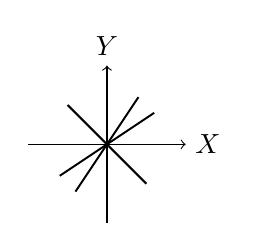
\begin{tikzpicture}
            \draw[->] (-1,0) -- (1,0) node[right] {$X$};
            \draw[->] (0,-1) -- (0,1) node[above] {$Y$};
            \draw[line width=0.25mm] (-0.4,-0.6) -- (0.4,0.6);
            \draw[line width=0.25mm] (-0.6,-0.4) -- (0.6,0.4);
            \draw[line width=0.25mm] (-0.5,0.5) -- (0.5,-0.5);
        \end{tikzpicture}
    \end{center}
    \par
    If $\abs k < \infty$, then the lemma fails. For example, $V = k^2 = \bigcup_{v \in k^2} \{v\} = \bigcup_{0 \neq v \in k^2} \operatorname{span}\{v\}$ with $0 \neq \operatorname{span}(v) \lneq k^2 = V$. \par
    The same technique shows that can't replace $V_1,\cdots,V_n$ with $V_1,V_2,\cdots$ over $\bbQ$.
\end{example}

\begin{theorem}[Prime avoidence, general version]
    Let $\ffb_1,\cdots,\ffb_n, \ffa \leq R$. Assume
    \begin{enumerate}
        \item $R$ contains an infinite field $k$ as a subring, or
        \item $\ffb_3,\cdots,\ffb_n \in \operatorname{Spec}(R)$.
    \end{enumerate}
    Then if $\ffa \not \subseteq \ffb_i$ for all $i = 1,\cdots,n$, then $\ffa \not \subseteq \bigcup_{i=1}^n \ffb_i$.
\end{theorem}

\begin{proof}
    \begin{enumerate}
        \item For each $i = 1,\cdots,n$, since $\ffa \not \subseteq \ffb_i$, $\ffa \cap \ffb_i \lneq \ffa$. Also, since $\ffa$ is a $k$-vector space, by Lemma 1.48, $\ffa \cap \bigcup_{i=1}^n \ffb_i = \bigcup_{i=1}^n (\ffa \cap \ffb_i) \lneq \ffa$. So $\ffa \not \subseteq \bigcup_{i=1}^n \ffb_i$. 
        \item Induct on $n$. Base case $n = 1$: done. Base case $n = 2$. Let $a_i \in \ffa \setminus \ffb_i$ for $i = 1,2$. Then $a_1 + a_2 \in \ffa$. Suppose $\ffa \subseteq \ffb_1 \cup \ffb_2$. Then $a_1 + a_2 \in \ffb_1 \cup \ffb_2$, say $a_1 + a_2 \in \ffb_2$. Since $a_1 \in \ffa \subseteq \ffb_1 \cup \ffb_2$ and $a_1 \not \in \ffb_1$, $a_1 \in \ffb_2$. So $a_2 = (a_1 + a_2) - a_1 \in \ffb_2$, a contradiction. \par 
            Induction step $n \geq 3$. Let $\ffa \not \subseteq \ffb_i$ for $i = 1,\cdots,n$. Assume $\ffa \not \subseteq \bigcup_{i \neq j} \ffb_i$ for $j = 1,\cdots,n$. Then there exists $a_j \in \ffa \setminus \{\bigcup_{i \neq j} \ffb_i\}$ for $j = 1,\cdots,n$. By way of contradiction, suppose $\ffa \subseteq \bigcup_{i=1}^n \ffb_i$. Then $a_j \in \bigcup_{i=1}^n \ffb_i \setminus \{\bigcup_{i \neq j}\ffb_i\} \subseteq \ffb_j$ for $j = 1,\cdots,n$. Note $a_1 \cdots a_{n-1} + a_n \in \ffa \subseteq \bigcup_{i=1}^n \ffb_i$. So there exists $l \in \{1,\cdots,n\}$ such that $a_1 \cdots a_{n-1} + a_n \in \ffb_l$. Suppose $l=n$. Since $a_n \in \ffb_n$, $a_1 \cdots a_{n-1} \in \ffb_n$. Since $n \geq 3$, we have $\ffb_n \in \operatorname{Spec}(R)$ and then $a_i \in \ffb_n$ for some $1 < i < n$, a contradiction. Hence we must have $l < n$. But since $a_1 \cdots a_l \cdots a_{n-1} \in \ffb_l$, we have $a_n \in \ffb_l$, a contradiction. \qedhere
    \end{enumerate}
\end{proof}

\begin{theorem}[Prime avoidence]
    Let $\ffp_1,\cdots,\ffp_n \in \operatorname{Spec}(R)$. If $\ffa \subseteq \bigcup_{i=1}^n \ffp_i$, then $\ffa \subseteq \ffp_i$ for some $i \in \{1,\cdots,n\}$, i.e., if $\ffa \not \subseteq \ffp_i$ for $i = 1,\cdots,r$, then $\ffa \not \subseteq \bigcup_{i=1}^n \ffp_i$.
\end{theorem}

\begin{fact*}[Avoidence for monomial ideals] 
    Let $A$ be a nonzero commutative ring with identity and $\ffa,\ffb_1,\cdots,\ffb_n$ be monomial ideals of $A[X_1,\cdots,X_d]$. If $\ffa \subseteq \bigcup_{i=1}^n \ffb_i$, $\ffa \subseteq \ffb_i$ for some $i \in \{1,\cdots,n\}$.
\end{fact*}

\begin{proof}
     By Dickson's lemma, $\ffa = \langle f_1,\cdots,f_m \rangle$ for some monomials $f_1,\cdots,f_m \in A[X_1,\cdots,X_d]$. Then $f_1 + \cdots + f_m \in \ffa \subseteq \bigcup_{i=1}^n \ffb_i$. So $f_1 + \cdots + f_m \in \ffb_i$ for some $i \in \{1,\cdots,n\}$. But $\ffb_i$ is a monomial ideal, so $f_1,\cdots,f_m \in \ffb_i$. Thus, $\ffa = \langle f_1,\cdots,f_m \rangle \subseteq \ffb_i$.
\end{proof}


\subsection*{Colon Ideals}
\addcontentsline{toc}{subsection}{Colon Ideals}

\begin{definition}
    Let $S \subseteq R$. Let 
    \begin{enumerate}
        \item 
            \[(\ffa:S) = \{r \in R \mid rs \in R, \fa s \in S\}.\]
        \item
            \[(0:S) = \{r \in R \mid rs = 0, \fa s \in S\} = \operatorname{Ann}_R(S).\]
    \end{enumerate}
\end{definition}

\begin{example}
    Let $R = k[X,Y]$. 
    \begin{enumerate}
        \item $(\langle XY \rangle: \{X,Y\}) = (\langle XY \rangle: \langle X,Y \rangle) = (\langle XY \rangle: \langle X \rangle) \bigcap (\langle XY \rangle: \langle Y \rangle) = \langle Y \rangle \bigcap \langle X \rangle= \langle XY \rangle$.
        \item
            \begin{align*}
                (\langle X^2,XY \rangle: \{X,Y\}) &= (\langle X^2,XY \rangle: \langle X,Y \rangle) = \left((\langle X^2 \rangle: \langle X \rangle) + (\langle X^2 \rangle: \langle Y \rangle)\right) \\
                &\textstyle \bigcap\left((\langle XY \rangle: \langle X \rangle)+(\langle XY \rangle: \langle Y \rangle)\right) = (\langle X \rangle + \langle X^2 \rangle) \textstyle \bigcap (\langle Y \rangle + \langle X \rangle) \\
                &= \langle X \rangle \textstyle \bigcap \langle X,Y \rangle = \langle X,XY \rangle = \langle X \rangle.
            \end{align*}
    \end{enumerate}
\end{example}

\begin{fact}
    Let $S \subseteq R$.
    \begin{enumerate}
        \item $\ffa \subseteq (\ffa:S) \leq R$.
        \item $(\ffa:\ffb)\ffb \subseteq \ffa$. 
        \item If $S \subseteq T$, then $(\ffa:S) \supseteq (\ffa:T)$.
        \item If $\ffa \subseteq \ffb$, then $(\ffa:S) \subseteq (\ffb:S)$.
        \item $(\ffa:S) = (\ffa:\langle S \rangle)$.
        \item $\ffb \subseteq \ffa$ if and only if $(\ffa:\ffb) = R$.
        \item $(\ffa: \bigcup_{\lambda \in \Lambda}S_\lambda) = \bigcap_{\lambda \in \Lambda} (\ffa:S_\lambda)$.
        \item $(\ffa: \sum_{\lambda \in \Lambda}\ffb_\lambda) = (\ffa: \bigcup_{\lambda \in \Lambda} \ffb_\lambda) = \bigcap_{\lambda \in \Lambda}(\ffa: \ffb_\lambda)$.
        \item $(\bigcap_{\lambda}\ffa_\lambda:S) = \bigcap_{\lambda \in \Lambda}(\ffa_\lambda:S)$.
        \item $((\ffa:\ffb):\ffc) = (\ffa:\ffb\ffc) = ((\ffa:\ffc):\ffb)$.
    \end{enumerate}
\end{fact}

\begin{proof}
    \begin{enumerate}
        \item[(b)]
            For each $r \in (\ffa:\ffb)$ and each $b \in \ffb$, we have $br \in \ffa$. It then follows from Fact 1.12.
        \item[(e)]
            ``$\supseteq$''. Since $S \subseteq \langle S \rangle$, by (c), $(\ffa:S) \supseteq (\ffa:\langle S \rangle)$. ``$\subseteq$''. Let $r \in (\ffa:S)$. Then $rs \in \ffa$ for any $s \in S$. Let $s \in \langle S \rangle$. Then $s = \sum_{i}^{\text{finite}}a_is_i$ for some $a_i \in R$ and $s_i \in S$ for each $i$. So $rs = r(\sum_i^{\text{finite}}a_is_i) = \sum_i^{\text{finite}} a_i(rs_i) \in R$. Hence $r \in (\ffa:\langle S \rangle)$.
        \item[(h)] This follows from (e) and (g).
        \item [(j)]
            It is enough to prove the first equality since $\ffb\ffc = \ffc\ffb$. Note $r \in ((\ffa:\ffb):\ffc)$ if and only if $rc \in (\ffa:\ffb)$ for any $c \in \ffc$ if and only if $r(bc) = (rc)b \in \ffa$ for any $b \in \ffb$ and $c \in \ffc$ if and only if $r \in (\ffa:\ffb\ffc)$ by (e). \qedhere
    \end{enumerate}
\end{proof}

\begin{example}
    Let $R = k[X,Y]$. It is straightforward to show the followings.
    \begin{enumerate}
        \item $(\langle XY \rangle: \langle X,Y \rangle) = (\langle XY \rangle: \{X,Y\}) = (\langle XY \rangle: X) \cap (\langle XY \rangle : Y) = \langle Y \rangle \cap \langle X \rangle = \langle XY \rangle$.
        \item $(\langle X^2,XY \rangle: \langle X,Y \rangle) = (\langle X^2,XY \rangle: \{X,Y\}) = (\langle X^2,XY \rangle:X) \cap (\langle X^2,XY \rangle: Y) = \langle X,Y \rangle$ \\
            $\cap \langle X \rangle = \langle X \rangle$.
    \end{enumerate}
\end{example}

\subsection*{Radicals of Ideals}
\addcontentsline{toc}{subsection}{Radicals of Ideals}

\begin{definition}
    The \emph{radical} of $\ffa \leq R$ is 
    \[\operatorname{rad}(\ffa) = \operatorname{r}(\ffa) = \sqrt \ffa = \{x \in R \mid x^n \in \ffa, \fa n \gg 0\} = \{x \in R \mid x^n \in \ffa \text{ for some }n \geq 1\}.\] 
\end{definition}

\begin{remark}
    $\operatorname{rad}(0) = \operatorname{Nil}(R)$.
\end{remark}

\begin{example}
    In $R = k[X,Y]$, we have
    \begin{align*}
        \operatorname{rad}(\langle X^2Y,XY^2 \rangle) &= \operatorname{m-rad}(\langle X^2Y,XY^2 \rangle) = \operatorname{m-rad}(\langle X^2Y \rangle + \langle XY^2 \rangle) \\
                                                      &= \operatorname{m-rad}(\langle X^2Y \rangle) + \operatorname{m-rad}(\langle XY^2 \rangle) = \langle XY \rangle + \langle XY \rangle = \langle XY \rangle.
    \end{align*}
\end{example}

\begin{fact}
    Let $\pi: R \to R/\ffa$ be the natural projection.
    \begin{enumerate}
        \item $\operatorname{rad}(\ffa) = \pi^{-1}(\operatorname{Nil}(R/\ffa)) \leq R$. 
        \item If $\ffa \subseteq \ffb$, then $\operatorname{rad}(\ffa) \subseteq \operatorname{rad}(\ffb)$. 
        \item $\ffa \subseteq \operatorname{rad}(\ffa) = \operatorname{rad}(\operatorname{rad}(\ffa))$. 
        \item $\operatorname{rad}(\ffa\ffb) = \operatorname{rad}(\ffa \cap \ffb) = \operatorname{rad}(\ffa) \cap \operatorname{rad}(\ffb)$.
        \item $\operatorname{rad}(\ffa) = R$ if and only if $\ffa = R$.
        \item $\operatorname{rad}(\ffa + \ffb) = \operatorname{rad}(\operatorname{rad}(\ffa) + \operatorname{rad}(\ffb))$.
        \item $\operatorname{rad}(\ffa) = \bigcap_{\ffp \in \operatorname{V}(\ffa)} \ffp$. 
        \item $\operatorname{rad}(\bigcap_{i=1}^n \ffp_i^{e_i}) = \bigcap_{i=1}^n \ffp_i$, where $\ffp_i \in \operatorname{Spec}(R)$ and $e_i \geq 1$ for $i = 1,\cdots,n$.
        \item $\ffa + \ffb = R$ if and only if $\operatorname{rad}(\ffa) + \operatorname{rad}(\ffb) = R$. 
    \end{enumerate}
\end{fact}

\begin{proof}
    \begin{enumerate}
        \item Let $r \in R$. Then $r \in \pi^{-1}(\operatorname{Nil}(R/\ffa))$ if and only if $\pi(r) \in \operatorname{Nil}(R/\ffa)$ if and only if $\overbar r^n = 0$ in $R/\ffa$ for some $n \geq 1$ if and only if $r^n \in \ffa$ for some $n \geq 1$ if and only if $r \in \operatorname{rad}(\ffa)$.
        \item It is straightforward.
        \item Since $a^1 = a \in \ffa$ for any $a \in \ffa$, we have $a \in \operatorname{rad}(\ffa)$ for any $a \in \ffa$. So $\ffa \subseteq \operatorname{rad}(\ffa)$. Then by (b), $\operatorname{rad}(\ffa) \subseteq \operatorname{rad}(\operatorname{rad}(\ffa))$. Let $r \in \operatorname{rad}(\operatorname{rad}(\ffa))$. Then there exists $n \geq 1$ such that $r^n \in \operatorname{rad}(\ffa)$. So there exists $m \geq 1$ such that $r^{mn} = (r^n)^m \in \ffa$. Hence $r \in \operatorname{rad}(I)$. 
        \item Since $\ffa\ffb \subseteq \ffa \cap \ffb \subseteq \ffa,\ffb$, by (b), we have $\operatorname{rad}(\ffa\ffb) \subseteq \operatorname{rad}(\ffa \cap \ffb) \subseteq \operatorname{rad}(\ffa),\operatorname{rad}(\ffb)$ and then $\operatorname{rad}(\ffa\ffb) \subseteq \operatorname{rad}(\ffa \cap \ffb) \subseteq \operatorname{rad}(\ffa) \cap \operatorname{rad}(\ffb)$. On the other hand, let $x \in \operatorname{rad}(\ffa) \cap \operatorname{rad}(\ffb)$. Then there exist $m,n \geq 1$ such that $x^m \in \ffa$ and $x^n \in \ffb$. So $x^{m+n} = x^m \cdot x^n \in \ffa \ffb$. Hence $x \in \operatorname{rad}(\ffa\ffb)$.
        \item $\ffa = R$ if and only if $1 \in \ffa$ if and only if $1^n \in \ffa$ if and only if $\operatorname{rad}(\ffa) = R$. 
        \item Since $\ffa + \ffb \subseteq \operatorname{rad}(\ffa) + \operatorname{rad}(\ffb)$, we have $\operatorname{rad}(\ffa + \ffb) \subseteq \operatorname{rad}(\operatorname{rad}(\ffa) + \operatorname{rad}(\ffb))$. \\
            Let $x \in \operatorname{rad}(\operatorname{rad}(\ffa) + \operatorname{rad}(\ffb))$. Then there exists $n \geq 1$ such that $x^n \in \operatorname{rad}(\ffa) + \operatorname{rad}(\ffb)$. So there exist $a \in \operatorname{rad}(\ffa)$ and $b \in \operatorname{rad}(\ffb)$ such that $x^n = a + b$. Then there exist $j,k \geq 1$ such that $a^j \in \ffa$ and $b^k \in \ffb$. So $x^{n(j+k)} = (x^n)^{j+k} = (a+b)^{j+k} = \sum_{l = 0}^{j+k} \binom{l}{j+k} a^lb^{j+k-l}$. Since for $0 \leq l \leq j+k$, either $l \geq j$ or $l < j$, i.e., $l \geq j$ or $j+k-l > k$, we have $a^l \in \ffa$ when $l \geq j$, and $b^{j+k-l} \in \ffb$ when $j + k - l > n$. So $x^{n(j+k)} = 0$. Thus, $x\in \operatorname{rad}(\ffa+\ffb)$.
        \item
            By Fact 1.15, $\operatorname{Spec}(R/\ffa) = \{\ffp/\ffa \mid \ffp \in \operatorname{V}(\ffa)\}$. So $\operatorname{Nil}(R/\ffa) = \bigcap_{\ffp \in \operatorname{Spec}(R/\ffa)} \ffp = \bigcap_{\ffp \in \operatorname{V}(\ffa)} \ffp/\ffa$. Then by (a), $\operatorname{rad}(\ffa) = \pi^{-1}(\operatorname{Nil}(R/\ffa))  = \pi^{-1}(\bigcap_{\ffp \in \operatorname{V}(\ffa)} \ffp/\ffa) = \bigcap_{\ffp \in \operatorname{V}(\ffa)} \pi^{-1}(\ffp/\ffa) = \bigcap_{\ffp \in \operatorname{V}(\ffa)} \ffp$.
        \item Since $\ffp_i \in \operatorname{Spec}(R)$, $\ffp_i \in \operatorname{V}(\ffp_i)$ and then $\ffp_i \subseteq \operatorname{rad}(\ffp_i) = \bigcap_{\ffp \in \operatorname{V}(\ffp_i)}\ffp \subseteq \ffp_i$, i.e., $\ffp_i = \operatorname{rad}(\ffp_i)$ for $i = 1,\cdots,n$. Then by (d), $\operatorname{rad}(\bigcap_{i=1}^n \ffp_i^{e_i}) = \bigcap_{i=1}^n \operatorname{rad}(\ffp_i^{e_i}) = \bigcap_{i=1}^n \operatorname{rad}(\ffp_i) = \bigcap_{i=1}^n \ffp_i$. 
        \item
            By (e) and (f), $\ffa + \ffb = R$ if and only if $\operatorname{rad}(\ffa + \ffb) = R$ if and only if $\operatorname{rad}(\operatorname{rad}(\ffa) + \operatorname{rad}(\ffb)) = R$ if and only if $\operatorname{rad}(\ffa) + \operatorname{rad}(\ffb) = R$. \qedhere
    \end{enumerate}
\end{proof}

\begin{example}
    \begin{enumerate}
        \item[(b)] Example of $\ffa \not \subseteq \ffb$ when $\operatorname{rad}(\ffa) \subseteq \operatorname{rad}(\ffb)$. Let $R = \bbZ$. Then $\operatorname{rad}(\langle 2 \rangle) = \langle 2 \rangle = \operatorname{rad}(\langle 4 \rangle)$, but $\langle 2 \rangle \not \subseteq \langle 4 \rangle$.
        \item[(c)]
            Example of $\ffa \subsetneq \operatorname{rad}(\ffa)$. Let $R = \bbZ$. Then $\langle 4 \rangle \subsetneq \langle 2 \rangle = \operatorname{rad}(\langle 4 \rangle)$.
        \item[(d)] Example of $\operatorname{rad}(\bigcap_{i=1}^\infty \ffa_i) \subsetneq \bigcap_{i=1}^\infty \operatorname{rad}(\ffa_i)$. Let $R = k[X_1,X_2,\cdots]$, $\ffa_1 = \langle X_1 \rangle$, $\ffa_2 = \langle X_1^2,X_2^2 \rangle$, $\cdots$, $\ffa_i = \langle X_1^i,\cdots,X_i^i \rangle$, $\cdots$. Since $\langle X_1,\cdots,X_i \rangle \in \operatorname{Spec}(R)$ for $i \geq 1$, by (f) and (g), we have $\operatorname{rad}(\ffa_i) = \operatorname{rad}(\langle X_1^i,\cdots,X_i^i \rangle) = \operatorname{rad}(\langle X_1,\cdots,X_i \rangle) = \langle X_1,\cdots,X_i \rangle$ for $i \geq 1$. So $\bigcap_{i=1}^\infty \operatorname{rad}(\ffa_i) = \bigcap_{i=1}^\infty \langle X_1,\cdots,X_i \rangle = \langle X_1 \rangle \supsetneq 0 = \operatorname{rad}(0) = \operatorname{rad}(\bigcap_{i=1}^\infty \ffa_i)$. 
        \item[(f)] Example of $\operatorname{rad}(\ffa + \ffb) \supsetneq \operatorname{rad}(\ffa) + \operatorname{rad}(\ffb)$. Let $R = k[X,Y]$, $\ffa = \langle X+Y^2 \rangle$ and $\ffb = \langle X \rangle$. Then $\ffa,\ffb \in \operatorname{Spec}(R)$. Also, since $\langle X,Y \rangle \in \operatorname{Spec}(R)$, $\operatorname{rad}(\ffa) + \operatorname{rad}(\ffb) = \ffa + \ffb = \langle X+Y^2,X \rangle = \langle X,Y^2 \rangle \subsetneq \langle X,Y \rangle = \operatorname{rad}(\langle X,Y^2 \rangle) = \operatorname{rad}(\ffa + \ffb)$.
    \end{enumerate}
\end{example}

\begin{example}
    \begin{enumerate}
        \item Let $R = \bbF_2[X,Y]$, $\ffa = \langle X,Y \rangle$, $\ffb_1 = \langle X,XY,Y^2 \rangle = \langle X,X^2,XY,Y^2 \rangle$, $\ffb_2 = \langle X+Y,X^2,Y^2 \rangle = \langle X+Y,X^2,XY,Y^2 \rangle$ and $\ffb_3 = \langle Y,X^2,XY \rangle = \langle Y,X^2,XY,Y^2 \rangle$. Then $\ffa \not \subseteq \ffb_i$ for $i = 1,2,3$. Let $f \in \ffa$. Then $f$ can be written as 
            \begin{align*}
                f &= X g(X) + X^2\alpha(X,Y) + XY\gamma(X,Y) + +Y^2\beta(X,Y) + Yh(Y) \\
                  &= X^2 \cdot \frac{g(X)-g(0)}{X} + (Xg(0)+Yh(0)) + Y^2 \cdot \frac{h(Y)-h(0)}{Y} \\
                  &\ \ \ + X^2\alpha(X,Y) + XY\gamma(X,Y) + Y^2\beta(X,Y).
            \end{align*}
            for some $g \in \bbF_2[X]$, $h \in \bbF_2[Y]$ and $\alpha,\beta,\gamma \in \bbF_2[X,Y]$. Since $g(0), h(0) \in \{0,1\}$, $f \in \ffb_1 \cup \ffb_2 \cup \ffb_3$. Also, since $\ffb_1 \cup \ffb_2 \cup \ffb_3 \subseteq \ffa$, we have $\ffa = \ffb_1 \cup \ffb_2 \cup \ffb_3$.
        \item Let $R = \frac{\bbF_2[X,Y]}{\langle X^2,XY,Y^2 \rangle}$ and $x = \overbar{X}, y = \overbar{Y} \in R$. Then $R \cong \bbF_2 \oplus \bbF_2x \oplus \bbF_2y$ and $\ffa := \langle x,y \rangle \cong \bbF_2x \oplus \bbF_2y$ as $\bbF_2$-vector space. Let $\ffb_1 = \langle x \rangle$, $\ffb_2 = \langle x + y \rangle$ and $\ffb_3 = \langle y \rangle$. Then $\ffa \not \subseteq \ffb_i$ for $i = 1,2,3$, but $\ffa = \ffb_1 \cup \ffb_2 \cup \ffb_2$.
    \end{enumerate}
\end{example}

\section*{Extensions and Contractions}
\addcontentsline{toc}{section}{Extensions and Contractions}

\begin{definition}
    Let $f: R \to S$ be a ring homomorphism. Let $\ffa \leq R$ and $\ffb \leq S$. The \emph{extension} of $\ffa$ along $f$ is 
    \[\ffa^e = \ffa S = \langle f(\ffa) \rangle S  = f(\ffa)S = \left\{\sum_i^{\text{finite}} f(a_i)s_i \mathrel{\Big |} a_i \in \ffa,\ s_i \in S, \fa i \right\} \leq S.\]
    The \emph{contraction} of $\ffb$ along $f$ is 
    \[\ffb^c = f^{-1}(\ffb) \leq R.\]
\end{definition}

\begin{example}
    \begin{enumerate}
        \item[(a)] Let $R$ be an integral domain with the field of fraction $Q(R)$. Then $R \subseteq Q(R)$ with the inclusion map $\epsilon:R \to Q(R)$ given by $\varepsilon(r) = r/1$. Note $0Q(R) = 0$ and $\ffa Q(R) = Q(R)$ for $0 \neq \ffa \leq R$.
        \item[(b)] Note $\langle X\rangle k[X] \subseteq k[X] \subseteq k[X,Y]$, $\left(\langle X \rangle k[X]\right)k[X,Y] = \langle X \rangle k[X,Y]$.
        \item[(c)] Let $R \subseteq S$ be rings and $\varepsilon: R \xrightarrow \subseteq S$. If $\ffb \leq S$, then $\varepsilon^{-1}(\ffb) = \ffb \cap R$.
        \item[(d)] Let $\varepsilon : k[X] \xrightarrow{\subseteq} k[X,Y]$. Since $\langle X,Y \rangle k[X,Y] \leq k[X,Y]$, we have $\varepsilon^{-1}(\langle X,Y \rangle k[X,Y]) = \langle X,Y \rangle k[X,Y] \textstyle \bigcap k[X] = \langle X \rangle k[X]$.
    \end{enumerate}
\end{example}

\begin{proposition}
    Let $f: R \to S$ be a ring homomorphism and $\ffb,\ffb_1,\ffb_2 \leq S$.
    \begin{enumerate}
        \item $\ffa \subseteq f^{-1}(\ffa S)$ and $f^{-1}(\ffb)S \subseteq \ffb$. If $\ffa_1 \subseteq \ffa_2$, then $\ffa_1S \subseteq \ffa_2S$. If $\ffb_1 \subseteq \ffb_2$, then $f^{-1}(\ffb_1) \subseteq f^{-1}(\ffb_2)$. If $T \subseteq R$, then $(\langle T \rangle R) S = \langle f(T) \rangle S$. \par
            Example of $\ffa \subsetneq f^{-1}(\ffa S)$. Let $f: R = \bbZ \xrightarrow {\subseteq} S = \bbQ$ and $\ffa = \langle 2 \rangle R$. Then $f^{-1}(\ffa S) = f^{-1}(S) = R \supsetneq \langle 2 \rangle R = \ffa$. \par 
            Example of $f^{-1}(\ffb)S \subsetneq \ffb$. Let $f: R = k[X] \xrightarrow {\subseteq } S = k[X,Y]$. Let $\ffb = \langle Y \rangle S$. Then $f^{-1}(\ffb) = 0$ and so $f^{-1}(\ffb)S = 0 \subsetneq \langle Y \rangle S = \ffb$.
        \item $\ffa S = f^{-1}(\ffa S)S$ and $f^{-1}(\ffb) = f^{-1}(f^{-1}(\ffb)S)$.
        \item $(\ffa_1 + \ffa_2)S = \ffa_1S + \ffa_2S$ and $f^{-1}(\ffb_1) + f^{-1}(\ffb_2) \subseteq f^{-1}(\ffb_1 + \ffb_2)$. \par 
            Example of $f^{-1}(\ffb_1) + f^{-1}(\ffb_2) \subsetneq f^{-1}(\ffb_1+\ffb_2)$. Let $f: R = k \xrightarrow \subseteq S = k[X]$, $\ffb_1 = \langle X \rangle S$ and $\ffb_2 = \langle X+1 \rangle S$. Then $f^{-1}(\ffb_1) = 0 = f^{-1}(\ffb_2)$ and so $f^{-1}(\ffb_1) + f^{-1}(\ffb_2) = 0 \subsetneq R = f^{-1}(S) = f^{-1}(\ffb_1 + \ffb_2)$.
        \item $(\ffa_1 \cap \ffa_2)S \subseteq \ffa_1S \cap \ffa_2S$ and $f^{-1}(\ffb_1 \cap \ffb_2) = f^{-1}(\ffb_1) \cap f^{-1}(\ffb_2)$. \par
            Example of $(\ffa_1 \cap \ffa_2)S \subsetneq \ffa_1S \cap \ffa_2S$. Let $f: R = k[X,Y] \to S = k[X,Y]/\langle X,Y \rangle^2$, $\ffa_1 = \langle X \rangle R$ and $\ffa_2 = \langle X+Y^2 \rangle R$. Then $\ffa_1 \cap \ffa_2 = \langle X(X+Y^2) \rangle R = \langle X^2 + XY^2 \rangle R$, $\ffa_1 S = \langle \overbar X \rangle S$ and $\ffa_2 S = \langle \overbar{X+Y^2} \rangle S = \langle \overbar X \rangle S$. So $(\ffa_1 \cap \ffa_2)S = \langle \overbar{X^2+XY^2} \rangle S = 0 \subsetneq \langle \overbar X \rangle S = \ffa_1 S \cap \ffa_2 S$.
        \item $(\ffa_1\ffa_2)S = (\ffa_1S)(\ffa_2S)$ and $f^{-1}(\ffb_1)f^{-1}(\ffb_2) \subseteq f^{-1}(\ffb_1\ffb_2)$. \par
            Example of $f^{-1}(\ffb_1)f^{-1}(\ffb_2) \subsetneq f^{-1}(\ffb_1\ffb_2) \subseteq f^{-1}(\ffb_1 \cap \ffb_2) = f^{-1}(\ffb_1) \cap f^{-1}(\ffb_2)$. Let $f: R = k[X] \to S = k[X]/(X(X-1)) = k[X]/(X^2-X) \cong k[X]/\langle X \rangle \times k[X]/\langle X-1 \rangle \cong k \times k$ by Chinese Remainder Theorem. Note in $k \times k$, $(1,0) = (1,0)^2$. Let $\ffb_1 = \langle \overbar X \rangle S = \ffb_2$. Then $\ffb_1 \ffb_2 = \langle \overbar X^2 \rangle S = \langle \overbar X \rangle S = \ffb_1$. So $f^{-1}(\ffb_1 \ffb_2) = f^{-1}(\ffb_1)  =  f^{-1}(\langle \overbar X \rangle S) = \langle X \rangle R \supsetneq \langle X^2 \rangle R = f^{-1}(\ffb_1)f^{-1}(\ffb_2)$.
        \item $(\ffa_1:\ffa_2)S \subseteq (\ffa_1S:\ffa_2S)$ and $f^{-1}(\ffb_1:\ffb_2) \subseteq (f^{-1}(\ffb_1):f^{-1}(\ffb_2))$. \par
            Example of $(\ffa_1:\ffa_2)S \subsetneq (\ffa_1S : \ffa_2 S)$. Let $f: R = k[X] \to S = k[X]/\langle X \rangle \cong k$, $\ffa_1 = \langle X^2 \rangle R$ and $\ffa_2 = \langle X \rangle R$. Then $\ffa_1 S = 0 = \ffa_2 S$ and so $(\ffa_1 S: \ffa_2 S) = (0:0) = S \supsetneq 0 = \langle X \rangle S = (\langle X^2 \rangle: \langle X \rangle)S = (\ffa_1:\ffa_2)S$. \par
            Example of $f^{-1}(\ffb_1:\ffb_2) \subsetneq (f^{-1}(\ffb_1):f^{-1}(\ffb_2))$. Let $f: R = k \xrightarrow {\subseteq} S = k[X]$, $\ffb_1 = \langle X \rangle S$ and $\ffb_2 = \langle X-1 \rangle S$. Then $(\ffb_1:\ffb_2) = (\langle X \rangle: \langle X-1 \rangle) = \langle X \rangle$ and $f^{-1}(\ffb_1) = 0 = f^{-1}(\ffb_2)$. So $f^{-1}(\ffb_1:\ffb_2) = f^{-1}(\langle X \rangle) = 0 \subsetneq R = (0:0) = (f^{-1}(\ffb_1):f^{-1}(\ffb_2))$. 
        \item $\operatorname{rad}(\ffa)S \subseteq \operatorname{rad}(\ffa S)$ and $f^{-1}(\operatorname{rad}(\ffb)) = \operatorname{rad}(f^{-1}(\ffb))$. \par
            Example of $\operatorname{rad}(\ffa) S \subsetneq \operatorname{rad}(\ffa S)$. Let $f: R = k[X] \to S = k[X]/\langle X^2 \rangle$ and $\ffa = 0R$. Then $\operatorname{rad}(\ffa)S = \operatorname{rad}(0R)S = 0S = 0 \subsetneq \langle \overbar X \rangle S = \operatorname{rad}(0S) = \operatorname{rad}(\ffa S)$.
    \end{enumerate}
\end{proposition}

\begin{proof}
    \begin{enumerate}
        \item 
            Note $\ffa \subseteq f^{-1}(f(\ffa)) \subseteq f^{-1}(f(\ffa) S) = f^{-1}(\ffa S)$. \par
            To show $\langle f(f^{-1}(\ffb)) \rangle S = f^{-1}(\ffb)S \subseteq \ffb$, it suffices to show $\langle f(f^{-1}(\ffb)) \rangle \subseteq \ffb$, then it is equivalent to show $f(f^{-1}(\ffb)) \subseteq \ffb$, which is true. \par 
            A set of generators of $(\langle T \rangle R)S$ over $S$ is 
            \[\left\{f\left(\sum_i^{\text{finite}}t_ir_i\right) = \sum_i^{\text{finite}} f(t_i)f(r_i) \mathrel{\bigg |} t_i \in T,\ r_i \in S, \fa i\right\} \subseteq \langle f(T) \rangle S.\] 
            \par A set of generators of $\langle f(T) \rangle S$ over $S$ is $\{f(t) \mid t \in T\} = \{f(t \cdot 1) \mid t \in T\}$ which is a subset of the generators of $(\langle T \rangle R)S$.
        \item 
            ``$\subseteq$''. By (a), $\ffa \subseteq f^{-1}(\ffa S)$, so $\ffa S \subseteq f^{-1}(\ffa S)S$. ``$\supseteq$''. A set of generators of $f^{-1}(\ffa S)S$ over $S$ is $\{f(x) \mid x \in f^{-1}(\ffa S)\} = f(f^{-1}(\ffa S)) \subseteq \ffa S$. \par
            ``$\subseteq$''. By (a), $\ffb \supseteq f^{-1}(\ffb)S$, so $f^{-1}(\ffb) \supseteq f^{-1}(f^{-1}(\ffb)S)$. ``$\subseteq$''. Let $x \in f^{-1}(\ffb)$. Then $f(x) = f(x) \cdot 1 \in \langle f(f^{-1}\ffb) \rangle S = f^{-1}(\ffb)S$. So $x \in f^{-1}(f^{-1}(\ffb)S)$.
        \item ``$\supseteq$''. Since $\ffa_1 + \ffa_2 \supseteq \ffa_1,\ffa_2$, we have $(\ffa_1+\ffa_2)S \supseteq \ffa_1S,\ffa_2S$. So $(\ffa_1+\ffa_2)S \supseteq \ffa_1S + \ffa_2S$. ``$\subseteq$''. A set of generators of $(\ffa_1+\ffa_2)S$ over $S$ is $\{f(a_1+a_2) = f(a_1) + f(a_2) \mid a_1 \in \ffa_1,a_2 \in \ffa_2\} \subseteq \ffa_1 S + \ffa_2 S$.         
        \item 
            Since $\ffa_1 \cap \ffa_2 \subseteq \ffa_1,\ffa_2$, $(\ffa_1 \cap \ffa_2)S \subseteq \ffa_1S,\ffa_2S$. So $(\ffa_1 \cap \ffa_2) S \subseteq \ffa_1 S \cap \ffa_2 S$. \par
            Note $x \in f^{-1}(\ffb_1 \cap \ffb_2)$ if and only if $f(x) \in \ffb_1 \cap \ffb_2$ if and only if $f(x) \in \ffb_1,\ffb_2$ if and only if $x \in f^{-1}(\ffb_1),f^{-1}(\ffb_2)$ if and only if $x \in f^{-1}(\ffb_1) \cap f^{-1}(\ffb_2)$.
        \item 
            ``$\subseteq$''. A set of generators of $(\ffa_1\ffa_2)S$ over $S$ is 
            \[\left\{f\left(\sum_i^{\text{finite}}\alpha_i\beta_i\right) = \sum_i^{\text{finite}} f(\alpha_i)f(\beta_i) \mathrel{\bigg |} \alpha_i \in \ffa_1,\ \beta_i \in \ffa_2, \fa i\right\} \subseteq (\ffa_1S)(\ffa_2S).\] 
            \par
            ``$\supseteq$''. Note 
            \begin{align*}
                (\ffa_1S)(\ffa_2S) &= (f(\ffa_1)S)(f(\ffa_2)S) = (f(\ffa_1)f(\ffa_2))S = \langle f(a_1)f(a_2) \mid a_1 \in \ffa_1,a_2 \in \ffa_2 \rangle S \\
                                   &= \langle f(a_1a_2) \mid a_1 \in \ffa_1,a_2 \in \ffa_2 \rangle S \subseteq \langle f(\ffa_1\ffa_2) \rangle S = (\ffa_1\ffa_2)S. 
            \end{align*}
        \item 
            A set of generators of $(\ffa_1:\ffa_2)S$ over $S$ is 
            \begin{align*}
                \{f(r) \mid r \in (\ffa_1:\ffa_2)\} &= \{f(r) \mid r \ffa_2 \subseteq \ffa_1\} \subseteq \{f(r) \mid r f(\ffa_2) \subseteq f(\ffa_1)\} \subseteq \{s \in S \mid sf(\ffa_2) \subseteq f(\ffa_1)\} \\
                                                    &= \{s \in S \mid s f(\ffa_2)S \subseteq f(\ffa_1)S \} = \{s \in S \mid s \ffa_2 S \subseteq \ffa_1 S\} = (\ffa_1S:\ffa_2S).
            \end{align*}
            \par Note 
            \begin{align*}
                f^{-1}(\ffb_1:\ffb_2) &= \{f^{-1}(s) \mid s \in (\ffb_1:\ffb_2)\} = \{f^{-1}(s) \mid s\ffb_2 \subseteq \ffb_1\} \subseteq \{f^{-1}(s) \mid sf^{-1}(\ffb_2) \\
                                      &\subseteq f^{-1}(\ffb_1)\} \subseteq \{r \in R\mid rf^{-1}(\ffb_2) \subseteq f^{-1}(\ffb_1)\} = (f^{-1}(\ffb_1):f^{-1}(\ffb_2)).
            \end{align*}
        \item 
            Let $s \in \operatorname{rad}(\ffa)S$. Then there exist $m \geq 1$, $a_i \in \operatorname{rad}(\ffa)$ and $s_i \in S$ for $i = 1,\cdots,m$ such that $s = \sum_{i=1}^m f(a_i)s_i$. Since $a_i \in \operatorname{rad}(\ffa)$, there exists $n_i \geq 1$ such that $a_i^{n_i} \in \ffa$ for $i = 1,\cdots,m$. Let $n = n_1 + \cdots + n_m$. Note if $k_1 + \cdots + k_m = n$ with $k_1,\cdots,k_m \geq 0$, then there exists some $i \in \{1,\cdots,m\}$ such that $k_i \geq n_i$ and so $a_i^{k_i} \in \ffa$. Hence  
            \[s^n = \left(\sum_{i=1}^m f(a_i)s_i\right)^n = \sum_{k_1 + \cdots + k_m = n} \frac{n!}{k_1! \cdots k_m!} f(a_1^{k_1} \cdots a_m^{k_m}) s_1^{k_1} \cdots s_m^{k_m} \subseteq f(\ffa)S = \ffa S.\]
            Thus, $s \in \operatorname{rad}(\ffa S)$. \par
            Note $x \in f^{-1}(\operatorname{rad}(\ffb))$ if and only if $f(x) \in \operatorname{rad}(\ffb)$ if and only if $f(x^n) = f(x)^n \in \ffb$ for some $n \geq 1$ if and only if $x^n  \in f^{-1}(\ffb)$ for some $n \geq 1$ if and only if $x \in \operatorname{rad}(f^{-1}(\ffb))$. \qedhere
    \end{enumerate}
\end{proof}

\begin{proposition}
    $R^\times + \operatorname{Nil}(R) \subseteq R^\times$. For any $u \in R^\times$ and any $x \in \operatorname{Nil}(R)$, we have $u+x \in R^\times$. For example, $1+x \in R^\times$.
\end{proposition}

\begin{proof}
    For any $y \in \operatorname{Nil}(R)$, there is a $n \geq 1$ such that $y^n = 0$, so $(1-y+y^2-\cdots+(-1)^{n-1}y^{n-1})(1+y) = 1-y^n = 1$, hence $1+y \in R^\times$. \par 
    Let $u \in R^\times$ and $x \in \operatorname{Nil}(R)$. Then $u^{-1}x \in \operatorname{Nil}(R)$. So $1+u^{-1}x \in R^\times$. Thus, $u + x = u(1+(u^{-1}x)) \in R^\times$. 
\end{proof}

\section*{Power Series Rings}
\addcontentsline{toc}{section}{Power Series Rings}

Let $A$ be a nonzero commutative ring with identity.

\begin{definition}
    \[A \llbracket X \rrbracket = \{f = \sum_{i=0}^\infty a_iX^i \mid a_i \in A, \fa i \geq 0\} \cong \prod_{i=0}^\infty A\] 
    with addition and multiplication defined by $(\sum_{i=0}^\infty a_iX^i) + (\sum_{i=0}^\infty b_iX^i) = \sum_{i=0}^\infty (a_i+b_i)X^i$ and $(\sum_{i=0}^\infty a_iX^i)(\sum_{i=0}^\infty b_iX^i) = \sum_{i=0}^\infty c_iX^i$, where $c_i = \sum_{j=0}^i a_jb_{i-j} = \sum_{p+q = i}a_pb_q$ for $i \geq 0$. Then $A\llbracket X \rrbracket$ is called a \emph{power series ring} with $0_{A\llbracket X \rrbracket} = 0_A = \sum_{i=0}^\infty 0_AX^i$ and $1_{A\llbracket X \rrbracket} = 1_A = 1_A + \sum_{i=0}^\infty 0_A X^i$. More generally, for any $\ffa \leq A$, $\ffa\llbracket X \rrbracket = \{\sum_{i=0}^\infty a_iX^i \mid a_i \in \ffa, \fa i \geq 0\}$.
\end{definition}

\begin{example}
    $e^X = \sum_{i=0}^\infty \frac{1}{i!} X^i \in \bbR \llbracket X \rrbracket$.
\end{example}

\begin{theorem}
    $A \llbracket X \rrbracket$ is a commutative ring with identity $1_A$ and $A \subseteq A[X] \subseteq A \llbracket X \rrbracket$ are subrings.
\end{theorem}

\begin{proposition}
    Let $f(X) = \sum_{i=0}^\infty a_iX^i$ with $a_i \in A$ for $i \geq 0$.
    \begin{enumerate}
        \item $f \in A \llbracket X \rrbracket^\times$ if and only if $a_0 \in A^\times$.
        \item If $\varphi: A \to B$ is a ring homomorphism, then there exists a well-defined ring homomorphism $\varphi\llbracket X \rrbracket: A\llbracket X \rrbracket \to B\llbracket X \rrbracket$ taking $\sum_{i=0}^\infty \alpha_iX^i$ to $\sum_{i=0}^\infty \varphi(\alpha_i)X^i$ and $A\llbracket X \rrbracket \geq \ker(\varphi \llbracket X \rrbracket) = \ker(\varphi)\llbracket X \rrbracket$. 
        \item For any $\ffa \leq A$, $\ffa \cdot A \llbracket X \rrbracket \subseteq \ffa \llbracket X \rrbracket \leq A\llbracket X \rrbracket$ and $A \llbracket X \rrbracket / \ffa \llbracket X \rrbracket \cong \frac{A}{\ffa} \llbracket X \rrbracket$. In addition, if $\ffa \leq A$ is finitely generated, $\ffa \cdot A\llbracket X \rrbracket = \ffa \llbracket X \rrbracket$.
        \item Let $\ffa \leq A$. Then 
            \[\langle X,\ffa \rangle A\llbracket X \rrbracket = X \cdot A \llbracket X \rrbracket + \ffa \cdot A \llbracket X \rrbracket = XA \llbracket X \rrbracket + \ffa \llbracket X \rrbracket = \left\{\sum_{i=0}^\infty b_iX^i \mathrel{\bigg |} b_0 \in \ffa,\ b_i \in A, \fa i \geq 1\right\} \leq A \llbracket X \rrbracket\] 
            and $A \llbracket X \rrbracket / \langle X,\ffa \rangle A \llbracket X \rrbracket \cong A/\ffa$. In particular, if $\ffa = 0$, then $\langle X \rangle A \llbracket X \rrbracket = \{\sum_{i=1}^\infty b_iX_i \mid b_i \in A, \fa i \geq 1\} \leq A\llbracket X \rrbracket$ and $A\llbracket X \rrbracket / \langle X \rangle A \llbracket X \rrbracket \cong A$. 
        \item If $f \in \operatorname{Nil}(A\llbracket X \rrbracket)$, then $a_i \in \operatorname{Nil}(A)$ for $i \geq 0$. The converse holds if $\langle a_0,a_1,a_2,\cdots \rangle$ is finitely generated. Also, $\operatorname{Nil}(A) \cdot A \llbracket X \rrbracket \subseteq \operatorname{Nil}(A \llbracket X \rrbracket) \subseteq \operatorname{Nil}(A) \llbracket X \rrbracket$.
        \item $f \in \operatorname{Jac}(A\llbracket X \rrbracket)$ if and only if $a_0 \in \operatorname{Jac}(A)$. Also, $\operatorname{Jac}(A\llbracket X \rrbracket) = \langle \operatorname{Jac}(A),X \rangle A\llbracket X \rrbracket$. 
        \item $A\llbracket X \rrbracket$ is an integral domain if and only if $A$ is an integral domain. Also, $A\llbracket X \rrbracket$ is never a field.
        \item $\ffa \leq A$ is prime if and only if $\ffa \llbracket X \rrbracket \leq A\llbracket X \rrbracket$ is prime if and only if $\langle \ffa,X \rangle A \llbracket X \rrbracket \leq A\llbracket X \rrbracket$ is prime. \par 
            Let $\epsilon: A \xrightarrow {\subseteq} A\llbracket X \rrbracket$. Then $\epsilon^*: \operatorname{Spec}(A\llbracket X \rrbracket) \to \operatorname{Spec}(A)$ taking $\ffp \llbracket X \rrbracket$ to $\epsilon^{-1}(\ffp\llbracket X \rrbracket)$ is always onto and never 1-1.
        \item $\ffa \leq A$ is maximal if and only if $\langle \ffa,X \rangle A \llbracket X \rrbracket \leq A \llbracket X \rrbracket$ is maximal. Also, $\ffa \llbracket X \rrbracket \leq A\llbracket X \rrbracket$ is never maximal.
        \item Let $\operatorname{m-Spec}(A\llbracket X \rrbracket) = \{\text{maximal ideals of}A\llbracket X \rrbracket\} \subseteq \operatorname{Spec}(A\llbracket X \rrbracket)$. Let $\ffm \in \operatorname{m-Spec}(A\llbracket X \rrbracket)$. Then 
            \begin{enumerate}
                \item $\ffm \cap A \in \operatorname{m-Spec}(A)$,
                \item $X \in \ffm$,
                \item $\ffm = \langle \ffm \cap A,X \rangle A\llbracket X \rrbracket$.
            \end{enumerate}
            \par Therefore,
            \begin{align*}
                \operatorname{m-Spec}(A) &\mathrel{\mathop{\rightleftarrows}^{\mathrm{\Lambda}}_{\mathrm{\epsilon^*}}} \operatorname{m-Spec}(A\llbracket X \rrbracket)  \\
                \ffn & \mapsto \langle \ffn,X \rangle A\llbracket X \rrbracket \\
                \ffm \cap A &\mapsfrom \ffm
            \end{align*}
    \end{enumerate}
\end{proposition}

\begin{proof}
    \begin{enumerate}
        \item 
            ``$\Rightarrow$''. Let $f \in A\llbracket X \rrbracket^\times$ with the multiplicative inverse $f^{-1}(X) = \sum_{i=0}^\infty b_iX^i \in A\llbracket X \rrbracket$ with $b_i \in A$ for $i \geq 0$. Then $1_A = f \cdot f^{-1} = (\sum_{i=0}^\infty a_iX^i)(\sum_{j=0}^\infty b_jX^j) = a_0b_0 + (a_0b_1 + a_1b_0)X + \cdots$. So $a_0b_0 = 1_A$ and hence $a_0 \in A^\times$. \par
            ``$\Leftarrow$''. We try to find $g = \sum_{j=0}^\infty b_iX^i \in A\llbracket X \rrbracket$ such that $fg = 1$, i.e., $1 = \sum_{i=0}^\infty (\sum_{j=0}^i a_jb_{i-j})X^i$. Then $a_0b_0 = 1$, $a_0b_1 + a_1b_0 = 0$, $a_0b_2 + a_1b_1 + a_2b_0= 0$, $\cdots$. If $a_0 = 1$, then $b_0 = a_0b_0 = 1$ and we can solve $b_n$ for $n \geq 1$ one by one, so $g$ is the inverse of $f$ and hence $f \in A\llbracket X \rrbracket$. If $a_0 \neq 1$, since $a_0b_0 = 1$, we have $a_0 \in A^\times $ and so by definition of multiplication in $A\llbracket X \rrbracket$,
            \[f = \sum_{i=0}^\infty a_iX^i = \sum_{i=0}^\infty a_0(a_0^{-1}a_i)X^i = a_0 \smallunderbrace{\left(1+\sum_{i=1}^\infty (a_0^{-1}a_i)X^i\right)}_{\in A\llbracket X \rrbracket^\times} \in A\llbracket X \rrbracket^\times.\]
        \item
            It is straightforward to show $\varphi \llbracket X \rrbracket$ is a well-defined ring homomorphism with
            \begin{align*}
                \ker(\varphi \llbracket X \rrbracket) &= \left\{\sum_{i=0}^\infty \alpha_i X^i \mathrel{\bigg |} \sum_{i=0}^\infty \varphi(\alpha_i)X^i = 0 \right\} = \left\{\sum_{i=0}^\infty \alpha_i X^i \mathrel{\bigg |} \varphi(\alpha_i) = 0, \fa i \geq 0\right\} \\
                                                      &= \left\{\sum_{i=0}^\infty \alpha_i X^i \mathrel{\bigg |} \alpha_i \in \ker(\varphi), \fa i \geq 0 \right\} = \ker(\varphi)\llbracket X \rrbracket.
            \end{align*}
        \item 
            Let $\tau: A \twoheadrightarrow A/\ffa$ be the natural projection. Then by (b), $\tau \llbracket X \rrbracket: A\llbracket X \rrbracket \to \frac{A}{\ffa}\llbracket X \rrbracket$ is a well-defined ring homomorphism with $A\llbracket X \rrbracket \geq \ker(\tau \llbracket X \rrbracket) = \ker(\tau) \llbracket X \rrbracket = \ffa \llbracket X \rrbracket$. Since $\tau$ is onto, by the first isomorphism theorem, $A\llbracket X \rrbracket / \ffa \llbracket X \rrbracket \cong \frac{A}{\ffa}\llbracket X \rrbracket$. Since $\ffa \subseteq \ker(\tau \llbracket X \rrbracket)$, we have $\langle \ffa \rangle A \llbracket X \rrbracket \subseteq \ker(\tau \llbracket X \rrbracket) = \ffa \llbracket X \rrbracket$. \par
            In addition, assume $\ffa = (\alpha_1,\cdots,\alpha_n)A$ for some $\alpha_1,\cdots,\alpha_n \in \ffa$. Let $f \in \ffa \llbracket X \rrbracket$. Then $a_i \in \ffa = (\alpha_1,\cdots,\alpha_n)A$ for $i \geq 0$. So for $i \geq 0$, we have $a_i = \sum_{j=1}^n b_{ij}\alpha_j$ for some $b_{i1},\cdots,b_{in} \in A$. Hence by the definition of addition and multiplication in $A\llbracket X \rrbracket$, 
            \[f = \sum_{i=0}^\infty a_iX^i = \sum_{i=0}^\infty \left(\sum_{j=1}^n b_{ij}\alpha_j\right)X^i = \sum_{j=1}^n \left(\sum_{i=0}^\infty \alpha_jb_{ij}X^i\right) = \sum_{j=1}^n \alpha_j \left(\sum_{i=0}^\infty b_{ij}X^i\right) \in \langle \ffa \rangle A\llbracket X \rrbracket.\]
        \item 
            Note
            \begin{center}
                \begin{tikzcd}
                    A\llbracket X \rrbracket \ar[rrr,"\pi"] \ar[ddd,swap,"\tau\llbracket X \rrbracket"] &[-32pt] & &[-22pt] A \ar[ddd,"\tau"] \\ [-15pt]
                    & \sum_{i=0}^{\infty} b_iX^{i} \ar[r,mapsto] \ar[d,mapsto] & b_0 \ar[d,mapsto] \\
                    & \sum_{i=0}^{\infty} \overbar{b}_iX^{i} \ar[r,mapsto] & \overbar{b}_0 \\ [-15pt] 
                    \frac{A}{\ffa}\llbracket X \rrbracket \ar[rrr,swap,"\pi'"] & & & \frac{A}{\ffa}
                \end{tikzcd}
            \end{center}
            \par It is straightforward to show $\pi$ and $\pi^{-1}$ are well-defined ring epimorphisms and the diagram commutes. \par 
            Note 
            \[\ker(\pi) = \left\{\sum_{i=1}^\infty b_iX^i \mathrel{\bigg |} b_i \in A, \fa i \geq 1\right\} = X\left\{\sum_{i=0}^\infty b_{i+1}X^i \mathrel{\bigg |} b_{i+1} \in A, \fa i \geq 0\right\} = X \cdot A \llbracket X \rrbracket.\]
            \par In general, 
            \[A\llbracket X \rrbracket \geq \ker(\tau \circ \pi) = \left\{\sum_{i=0}^\infty b_iX^i \mathrel{\bigg |} b_0 \in \ffa,\ b_i \in A, \fa i \geq 1\right\} =: I.\]
            \par Let $\sum_{i=0}^\infty b_i X^i \in I$ with $b_0 \in \ffa$ and $b_i \in A$ for $i \geq 1$. Then $\sum_{i=0}^\infty b_iX^i = b_0 + X \sum_{i=0}^\infty b_{i+1}X^i$ \\
            $\in \ffa + X A\llbracket X \rrbracket \subseteq \langle X,\ffa \rangle A\llbracket X \rrbracket$. So $I \subseteq \langle X,\ffa \rangle A\llbracket X \rrbracket$. \par 
            Since $X = 0 + 1 \cdot X$ and $0 \in \ffa$ and $1\in A$, we have $X \in I \leq A\llbracket X \rrbracket$. Also, for $\sum_{i=0}^\infty b_iX^i \in \ffa \llbracket X \rrbracket$ \\
            $\leq A \llbracket X \rrbracket$ with $b_0 \in \ffa$ and $b_i \in \ffa \subseteq A$ for $i \geq 1$, we have $\sum_{i=0}^\infty b_iX^i \in I$ and so $\ffa \llbracket X \rrbracket \subseteq I$. Hence $\langle X \rangle A\llbracket X \rrbracket + \ffa\llbracket X \rrbracket \subseteq I$. \par
            Thus, by (c),
            \[\langle X,\ffa \rangle A\llbracket X \rrbracket \supseteq I \supseteq \langle X \rangle A\llbracket X \rrbracket + \ffa \llbracket X \rrbracket \supseteq \langle X \rangle A\llbracket X \rrbracket + \langle \ffa \rangle A\llbracket X \rrbracket = \langle X,\ffa \rangle A\llbracket X \rrbracket.\] 
            \par So $\langle X,\ffa \rangle A\llbracket X \rrbracket = \langle X \rangle A \llbracket X \rrbracket + \langle \ffa \rangle A\llbracket X \rrbracket = \langle X \rangle A\llbracket X \rrbracket + \ffa \llbracket X \rrbracket = I = \ker(\tau \circ \pi)$. By the first isomorphism theorem, $A\llbracket X \rrbracket / \langle X,\ffa \rangle A \llbracket X \rrbracket \cong A/\ffa$. 
        \item 
            Assume $f \in \operatorname{Nil}(A\llbracket X \rrbracket)$. Then $0 = f^n = a_0^n + Xg(X)$ for some $n \geq 1$ and $g \in A\llbracket X \rrbracket$. So $a_0^n = 0$ and then $a_0 \in \operatorname{Nil}(A) \subseteq \operatorname{Nil}(A\llbracket X \rrbracket)$. Hence $\sum_{i=1}^\infty a_iX^i = f-a_0 \in \operatorname{Nil}(A \llbracket X \rrbracket)$. Similarly, we have $a_1 \in \operatorname{Nil}(A\llbracket X \rrbracket)$. By induction, $a_i \in \operatorname{Nil}(A)$ for $i \geq 0$. \par 
            So we can conclude $\operatorname{Nil}(A\llbracket X \rrbracket) \subseteq \operatorname{Nil}(A)\llbracket X \rrbracket$. Furthermore, since $\operatorname{Nil}(A) \subseteq \operatorname{Nil}(A\llbracket X \rrbracket) \leq A \llbracket X \rrbracket$, we have $\operatorname{Nil}(A) = \operatorname{Nil}(\operatorname{Nil}(A)) \subseteq \operatorname{Nil}(A\llbracket X \rrbracket) \leq A\llbracket X \rrbracket$ and then $\operatorname{Nil}(A) \cdot A\llbracket X \rrbracket \subseteq \operatorname{Nil}(A\llbracket X \rrbracket)$. Thus, $\operatorname{Nil}(A) \cdot A\llbracket X \rrbracket \subseteq \operatorname{Nil}(A\llbracket X \rrbracket) \subseteq \operatorname{Nil}(A)\llbracket X \rrbracket$. \par 
            Assume $a_i \in \operatorname{Nil}(A)$ for $i \geq 0$ and $\langle a_0,a_1,\cdots \rangle$ is finitely generated. Then $\langle a_0,a_1,\cdots \rangle = \langle a_0,a_1,\cdots,a_t \rangle$ for some $t \geq 1$. So $f = \sum_{i=0}^\infty a_iX^i = \sum_{j=0}^t a_jf_j$, where $f_j \in \operatorname{Nil}(A) \cdot A \llbracket X \rrbracket \subseteq \operatorname{Nil}(A\llbracket X \rrbracket) \leq A\llbracket X \rrbracket$ for $j = 0,\cdots,t$. Thus, $f \in \operatorname{Nil}(A\llbracket X \rrbracket)$. 
        \item  ``$\Rightarrow$''. Assume $f \in \operatorname{Jac}(A\llbracket X \rrbracket)$. Then by Proposition 1.29, $1-fg \in A\llbracket X \rrbracket^\times$ for any $g \in A\llbracket X \rrbracket$. So $(1-a_0a) + a_1ax + a_2ax^2 + \cdots = 1-fa \in A\llbracket X \rrbracket^\times$ for any $a \in A$. Then by (a), $1-a_0a \in A^\times$ for any $a \in A$. Hence $a_0 \in \operatorname{Jac}(A)$ by Proposition 1.29. \par 
            ``$\Leftarrow$''. If $a_0 \in \operatorname{Jac}(A)$, then $1-a_0a \in A^\times$ for any $a \in A$. Let $g = \sum_{i=0}^\infty b_iX^i \in A\llbracket X \rrbracket$ with $b_i \in A$ for $i \geq 0$. To show $f \in \operatorname{Jac}(A\llbracket X \rrbracket)$. Need to show $1-fg \in A\llbracket X \rrbracket^\times$. By (a), it is equivalent to show the constant term of $1-fg$ is in $A^\times$. Note $1-fg = 1-(\sum_{i=0}^\infty a_iX^i)(\sum_{i=0}^\infty b_iX^i) = \smallunderbrace{(1-a_0b_0)}_{\in A^\times} + \cdots$. \par 
            Thus, $\operatorname{Jac}(A\llbracket X \rrbracket) = \{\sum_{i=0}^\infty a_iX^i \mid a_0 \in \operatorname{Jac}(A)\} = \langle \operatorname{Jac}(A),X \rangle A \llbracket X \rrbracket$ by (d). 
        \item 
            Define $\operatorname{ord}(f) = \inf\{i \geq 0 \mid a_i \neq 0\}$. Then $\operatorname{ord}(fg) \geq \operatorname{ord}(f) + \operatorname{ord}(g)$ with equality if, e.g., $A$ is an integral domain. \par 
            ``$\Leftarrow$''. Let $A$ be an integral domain and $f,g \neq 0$ in $A\llbracket X \rrbracket$. Then $\operatorname{ord}(f),\operatorname{ord}(g) \neq \infty$. So $\operatorname{ord}(fg) = \operatorname{ord}(f)\operatorname{ord}(g) \neq \infty$. Hence $fg \neq 0$. \par
            ``$\Rightarrow$''. Let $A\llbracket X \rrbracket$ be an integral domain. Since $0 \neq A$ is a subring of $A\llbracket X \rrbracket$, $A$ is also an integral domain. \par
            Since $X \in A\llbracket X \rrbracket$ and the constant term of $X$ is 0, which is not in $A^\times$, by (a), $X \not \in A\llbracket X \rrbracket^\times$. So $A\llbracket X \rrbracket$ is not a field.
        \item 
            Note $\ffa \leq A$ is prime if and only if $A/\ffa$ is an integral domain if and only if $\frac{A}{\ffa}\llbracket X \rrbracket$ is an integral domain by (g) if and only if $A\llbracket X \rrbracket/\ffa \llbracket X \rrbracket$ is an integral domain by (c) if and only if $\ffa\llbracket X \rrbracket \leq A \llbracket X \rrbracket$ is prime. \par 
            Note $\ffa \leq A$ is prime if and only if $A/\ffa$ is an integral domain if and only $\frac{A\llbracket X \rrbracket}{\langle X,\ffa \rangle A\llbracket X \rrbracket}$ is an integral domain by (d) if and only if $\langle \ffa,X \rangle A\llbracket X \rrbracket \leq A\llbracket X \rrbracket$ is prime. \par
            Let $\ffp \in \operatorname{Spec}(A)$. Then $\ffp\llbracket X \rrbracket, \langle \ffp,X \rangle A\llbracket X \rrbracket \in \operatorname{Spec}(A\llbracket X \rrbracket)$. \par 
            By the proof of (c) and (d), we have $\ffp \llbracket X \rrbracket \cap A = \ffp$ and $\langle \ffp,A \rangle A\llbracket X \rrbracket \cap A = \ffp$. So by Fact 1.16,
            \begin{align*}
                \epsilon^*(\ffp \llbracket X \rrbracket) & = \epsilon^{-1}(\ffp \llbracket X \rrbracket) = \ffp \llbracket X \rrbracket \cap A = \ffp = (\langle \ffp,A \rangle A\llbracket X \rrbracket) \cap A = \epsilon^{-1}(\langle \ffp,X \rangle A\llbracket X \rrbracket) = \epsilon^*(\langle \ffp,X \rangle A\llbracket X \rrbracket). 
            \end{align*}
            Thus, $\epsilon^*$ is onto. Also, since $X \not \in \ffp \llbracket X \rrbracket$, but $X \in \langle \ffp,X \rangle \llbracket X \rrbracket$, we have $\ffp\llbracket X \rrbracket \neq \langle \ffp,X \rangle A\llbracket X \rrbracket$ and then $\epsilon^*$ is not 1-1.
        \item 
            Note $\ffa \leq A$ is maximal if and only if $A/\ffa$ is a field if and only $A\llbracket X \rrbracket / \langle X,\ffa \rangle A\llbracket X \rrbracket$ is a field by (d) if and only if $\langle \ffa,X \rangle A\llbracket X \rrbracket \leq A\llbracket X \rrbracket$ is maximal. \par 
            Since $\frac{A}{\ffa}\llbracket X \rrbracket$ is not a field by (g), $A\llbracket X \rrbracket / \ffa \llbracket X \rrbracket$ is not a field by (c), then $\ffa \llbracket X \rrbracket \leq A\llbracket X \rrbracket$ is not maximal. 
        \item 
            \begin{enumerate}
                \item [(2)]
                    Since $X \in \operatorname{Jac}(A\llbracket X \rrbracket)$ by (f), and $\ffm \in \operatorname{m-Spec}(A\llbracket X \rrbracket)$, we have $X \in \ffm$. 
                \item [(1)]
                    By prime correspondence under quotients, we have $\ffm$ corresponds to a maximal ideal in $A\llbracket X \rrbracket/\langle X \rangle A \llbracket X \rrbracket \cong A$ by (d).
                    \begin{alignat*}{2}
                        A\llbracket X \rrbracket &\xrightarrow{\pi} A\llbracket X \rrbracket/\langle X \rangle A\llbracket X \rrbracket &&\xrightarrow \cong A \\
                        \ffm &\leadsto \ffm/\langle X \rangle A\llbracket X \rrbracket &&\leadsto \ffn
                    \end{alignat*}
                    Define $\tau: A\llbracket X \rrbracket \to A$ by $\tau(f) = f(0)$. Then we can find $\ffn \in \operatorname{m-Spec}(A)$ such that $\ffm = \tau^{-1}(\ffn)$. So 
                    \[\ffm \cap A = \epsilon^{-1}(\ffm) = \epsilon^{-1}(\tau^{-1} (\ffn)) = (\tau \circ \epsilon)^{-1}(\ffn) = \operatorname{id}_A^{-1}(\ffn) = \ffn \in \operatorname{m-Spec}(A).\]
                \item [(3)] Since $\ffm \cap A, \langle X \rangle \subseteq \ffm$, we have $\langle \ffm \cap A,X \rangle \subseteq \ffm$. Since $\ffm \leq A\llbracket X \rrbracket$ is maximal, and by (i) and (1), $\langle \ffm \cap A,X \rangle \leq A \llbracket X \rrbracket$ are maximal, we have $\langle \ffm \cap A,X \rangle = \ffm$.
            \end{enumerate} 
            \par Note $\epsilon^*(\operatorname{m-Spec}(A\llbracket X \rrbracket) \subseteq \operatorname{m-Spec}(A)$ since by the proof of (1), $\epsilon^*(\ffm) = \epsilon^{-1}(\ffm) \in \operatorname{m-Spec}(A)$. \par 
            Note $\Lambda (\operatorname{m-Spec}(A)) \subseteq \operatorname{m-Spec}(A\llbracket X \rrbracket)$ since by (i), $\Lambda(\ffn) = \langle \ffn,X \rangle A\llbracket X \rrbracket \in \operatorname{Spec}(A\llbracket X \rrbracket)$ for any $\ffn \in \operatorname{Spec}(A)$. \par 
            Note $\Lambda(\epsilon^*(\ffm)) = \Lambda (\epsilon^{-1}(\ffm)) = \Lambda (\ffm \cap A) = \langle \ffm \cap A,X \rangle A\llbracket X \rrbracket = \ffm$ by (3). \par 
            Note $\epsilon^*(\Lambda(\ffn)) = \epsilon^*(\langle \ffn,X \rangle A\llbracket X \rrbracket)= \epsilon^{-1}(\langle \ffn,X \rangle A\llbracket X \rrbracket) = \langle \ffn,X \rangle \cap A = \ffn$ by the proof of (c) for any $\ffn \leq \operatorname{m-Spec}(A)$. \par 
            Therefore, we have a 1-1 correspondence between $\operatorname{m-Spec}(A\llbracket X \rrbracket)$ and $\operatorname{m-Spec}(A)$.
        \qedhere
    \end{enumerate}
\end{proof}

\begin{example}
    \begin{enumerate}
        \item [(c)] Example of $\langle \ffa \rangle A\llbracket X \rrbracket \subsetneq \ffa\llbracket X \rrbracket$ for some $\ffa \leq A$. Let $A = k[Y_1,Y_2,Y_3,\cdots]$ and $\ffa = \langle Y_1,Y_2,Y_3,\cdots \rangle A$. Let $f = \sum_{i=1}^\infty Y_iX^i \in \ffa \llbracket X \rrbracket$. Claim. $f \not \in \langle \ffa \rangle A\llbracket X \rrbracket = \langle Y_1,Y_2,\cdots \rangle A\llbracket X \rrbracket$. Suppose $f \in \langle Y_1,Y_2,\cdots \rangle A\llbracket X \rrbracket$. Then there exists $m \geq 1$ and $\sum_{j=0}^\infty b_{ij}X^j = g_i \in A\llbracket X \rrbracket$ for $i = 1,\cdots,m$ such that $\sum_{j=1}^\infty Y_jX^j = f = \sum_{i=1}^m g_iY_i = \sum_{i=1}^m (\sum_{j=0}^\infty b_{ij}X^j)Y_i = \sum_{j=0}^\infty (\sum_{i=1}^m b_{ij}Y_i)X^j$. So for $j \geq 1$, we have $Y_j = \sum_{i=1}^m b_{ij}Y_i \in \langle Y_1,\cdots,Y_m \rangle A$. Then $Y_{m+1} \in \langle Y_1,\cdots,Y_m \rangle A$, a contradiction.
        \item [(e)]
            Example of $f \not \in \operatorname{Nil}(A\llbracket X \rrbracket)$ when $a_i \in \operatorname{Nil}(A)$ for $i \geq 0$. Let $A = \frac{\bbQ[Y_1,Y_2,Y_3,\cdots]}{\langle Y_1^2,Y_2^3,Y_3^4,\cdots,Y_i^{i+1},\cdots \rangle}$ and $a_0 = 0 \in \operatorname{Nil}(A)$ and $a_i = \overbar Y_i$ for $i \geq 1$. Then $a_i^{i+1} = \overbar{Y_i^{i+1}} = 0$ and so $a_i \in \operatorname{Nil}(A)$ for $i \geq 1$. \par 
            Claim. $f \not \in \operatorname{Nil}(A\llbracket X \rrbracket)$. Note $f^2 = (\sum_{i=1}^\infty \overbar Y_i X^i)^2 = \smallunderbrace{\overbar Y_1^2 X^2}_{= 0} + \smallunderbrace{(2\overbar Y_1 \overbar Y_2)X^3}_{\neq 0} + \cdots$, and $f^3 = (\sum_{i=1}^\infty \overbar Y_i X^i)^3 = \smallunderbrace{\overbar Y_1^3 X^3}_{= 0} + \smallunderbrace{(2\overbar Y_1 \overbar Y_3 + \overbar {Y_2^2})X^4}_{\neq 0} + \cdots$, and inductively, we find $f^n$ has lots of nonzero coefficients for $n \geq 1$.
    \end{enumerate}
\end{example}

\begin{definition}
    Define
    \[A\llbracket X,Y \rrbracket = A\llbracket X \rrbracket \llbracket Y \rrbracket,\]
    and for $d \geq 2$,
    \[A\llbracket X_1,\cdots,X_d \rrbracket = A \llbracket X_1,\cdots,X_{d-1} \rrbracket \llbracket X_d \rrbracket.\]
\end{definition}

\begin{fact}
    $A\llbracket X_1,\cdots,X_d \rrbracket = \{\sum_{\underline n \in \bbN_0^d} a_{\underline n} \underline X^{\underline n} \mid a_{\underline n} \in A\}$ for $d \geq 1$, where $\underline X^{\underline n} = X_1^{n_1} \cdots X_d^{n_d}$ and $\underline n = (n_1,\cdots,n_d) \in \bbN_0^d$.
\end{fact}

\begin{warning}
    The operations on $A\llbracket X_1,X_2,X_3,\cdots \rrbracket$ are ambiguous.
\end{warning}


\section*{U.F.D.}
\addcontentsline{toc}{section}{U.F.D.}

Let $k$ be a field.

\begin{definition}
    An integral domain is a U.F.D. if it is \emph{atomic} (every nonzero nonunit of $R$ can be factored into irreducibles) and given two irreducible factorizations $\alpha_1 \cdots \alpha_n = \beta_1 \cdots \beta_n$,
    \begin{enumerate}
        \item $n = m$,
        \item there exists $\sigma \in S_n$ such that $\alpha_i = u_i \beta_{\sigma(i)}$ with $u_i \in R^{\times}$ for $i = 1,\cdots,n$.
    \end{enumerate}
\end{definition}

\begin{example}
    Examples of UFD's: $k$, $\bbZ$, $\bbZ[i]$, $\bbZ[\frac{-1+\sqrt {-3}}{2}],\bbZ[\frac{-1+\sqrt{-19}}{2}]$, $k[X]$, $k\llbracket X \rrbracket$, $k[X_1,\cdots,X_n]$, $k\llbracket X_1,\cdots,X_n \rrbracket $ and $k\llbracket \{X_i\}_{i \in I} \rrbracket$.
\end{example}

\begin{definition}
    We say $x \in R$ is \emph{irreducible} if $x = ab$, then $a$ or $b$ is a unit.
\end{definition}

\begin{definition}
    We say $x \in R$ is \emph{prime} if $x$ is a nonunit and $x \mid a$ or $x \mid b$ whenever $x \mid ab$.
\end{definition}

\begin{example}
    Examples of non-UFD's:
    \begin{enumerate}
        \item 
            $\bbZ[\sqrt{-5}] = \{m+n\sqrt{-5} \mid m,n \in \bbZ\}$, where $6 = (2)(3) = (1+\sqrt {-5})(1-\sqrt{-5})$.
        \item
            $k[X^{2},X^{3}] = \{a_0+a_2X^{2}+a_3X^{3}+a_4X^{4}+\cdots + a_nx^{n} \mid n \geq 0, a_i \in k,\fa i = 0,2,3,\cdots,n\}$, where $X^{6} = X^{2} \cdot X^{2} \cdot X^{2} = X^{3} \cdot X^{3}$ with $X^{2}$ and $X^{3}$ irreducible here.
    \end{enumerate}
\end{example}

\begin{definition}
    An integral domain $R$ is a UFD if every nonzero nonunit element is a product of primes.
\end{definition}

\begin{theorem}
    If $R$ is a UFD, then so is 
    \begin{enumerate}
        \item $R[\{X_i\}_{i \in I}]$,
        \item $R_U$, where $0 \not \in U \subseteq R$ is multiplicatively closed.
    \end{enumerate}
\end{theorem}

\begin{fact}
    If $R$ is a UFD, it is integrally closed.
\end{fact}

\begin{theorem}
    Let $R$ be an integral domain. Then $R$ is a UFD if and only if every nonzero prime ideal contains some nonzeo prime element.
\end{theorem}

\begin{theorem}
    If $R$ is a PID, then $R\llbracket X \rrbracket$ is a UFD.
\end{theorem}

\begin{example}
    There exists some UFD's $R$ such that $R\llbracket X \rrbracket $ is not a UFD.
\end{example}

\begin{question}
    If $R\llbracket X \rrbracket$ is a UFD, is $R\llbracket X,Y \rrbracket$ a UFD? 
\end{question}

\begin{comment}

\section*{Exercises}

Let $R_1,R_2,\cdots$ be nonzero commutative rings with identity.

\begin{exer}
    The product $R_1 \times R_2$ is a nonzero commutative ring with identity where the operations and identities are defined component-wise: $(a_1,a_2) + (b_1,b_2) = (a_1+b_1,a_2+b_2)$ and $(a_1,a_2)(b_1,b_2) = (a_1b_1,a_2b_2)$ with $0_{R_1 \times R_2} = (0_{R_1},0_{R_2})$ and $1_{R_1 \times R_2} = (1_{R_1},1_{R_2})$. 
    \begin{enumerate}
        \item Prove that if $\ffa_1 \leq R_1$ and $\ffa_2 \leq R_2$, then use the first isomorphism theorem to show that $\ffa_1 \times \ffa_2 \leq R_1 \times R_2$ and $(R_1 \times R_2)/(\ffa_1 \times \ffa_2) \cong (R_1/\ffa_1) \times (R_2/\ffa_2)$.
        \item Prove that $R_1 \times R_2$ is not an integral domain. Conclude that if $\ffa_1 \lneq R_1$ and $\ffa_2 \lneq R_2$, then $(R_1/\ffa_1) \times (R_2/\ffa_2)$ is not an integral domain. 
        \item Prove that $\{\ffa \leq R_1 \times R_2\} = \{\ffa_1 \times \ffa_2 \mid \ffa_1 \leq R_1,\ \ffa_2 \leq R_2\}$.
        \item Prove that $\operatorname{Spec}(R_1 \times R_2)$ is the disjoint union of the sets $\{\ffp_1 \times R_2 \mid \ffp_1 \in \operatorname{Spec}(R_1)\}$ and $\{R_2 \times \ffp_2 \mid \ffp_2 \in \operatorname{Spec}(R_2)\}$.
        \item State and prove a characterization of the maximal ideals of $R_1 \times R_2$ as in part (d). In particular, conclude that $R_1 \times R_2$ is not local.
    \end{enumerate}
\end{exer}

\begin{proof}
    \begin{enumerate}
        \item Define $\phi: R_1 \times R_2 \to (R_1/\ffa_1) \times (R_2/\ffa_2)$ by $\phi(r_1,r_2) = (r_1+\ffa_1,r_2+\ffa_2)$. Let $(r_1,r_2),(s_1,s_2) \in R_1 \times R_2$. Then $\phi((r_1,r_2)+(s_1,s_2)) = \phi(r_1+s_1,r_2+s_2) = (r_1+s_1+\ffa_1,r_2+s_2+\ffa_2) = (r_1+\ffa_1,r_2+\ffa_2) + (s_1+\ffa_1,s_2+\ffa_2) = \phi(r_1,r_2) + \phi(s_1,s_2)$ and it is similar for the multiplication. So $\phi$ is a ring homomorphism. Note $(r_1,r_2) \in \ker(\varphi)$ if and only if $\phi(r_1,r_2) = 0$ if and only if $(r_1+\ffa,r_2+\ffa) = (\ffa_1,\ffa_2)$ if and only if $r_1 \in \ffa_1$ and $r_2 \in \ffa_2$. So $\ker(\varphi) = \ffa_1 \times \ffa_2$. Then our result follows from the first isomorphism theorem.
        \item Let $(0_{R_1},1_{R_2}),(1_{R_1},0_{R_2}) \in R_1 \times R_2$. Since $R_1 \neq 0 \neq R_2$, $(0_{R_1},1_{R_2}) \neq (0_{R_1},0_{R_2}) \neq  (1_{R_1},0_{R_2})$, but $(0_{R_1},1_{R_2}) \times (1_{R_1},0_{R_2}) = (0_{R_1},0_{R_2}) = 0_{R_1 \times R_2}$. So $R_1 \times R_2$ is not an integral domain. \\
            Since $\ffa_1 \lneq R_2$ and $\ffa_2 \lneq R_2$, $\ffa_1 \times \ffa_2 \lneq R_1 \times R_2$ . Suppose $(R_1 \times \ffa_1) \times (R_2/\ffa_2)$ is an integral domain. Then by (a), $(R_1 \times R_2)/(\ffa_1 \times \ffa_2)$ is an integral domain. Also, since $(R_1 \times R_2)/(\ffa_1 \times \ffa_2) \neq 0$, we have $R_1 \times R_2$ is an integral domain, a contradiction.
        \item ``$\supseteq$''. Follow from (a). ``$\subseteq$''. Let $\ffa = I \times J \leq R_1 \times R_2$, where $I \subseteq R_1$ and $J \subseteq R_2$. Then $(r_1i,r_2j) = (r_1,r_2)(i,j) \in I \times J$ for any $(r_1,r_2) \in R_1 \times R_2$ and $(i,j) \in I \times J$, i.e., for any $r_1 \in R_1,r_2 \in R_2,i \in I,j \in J$, we have $r_1i \in I$ and $r_2j \in J$. So $I \leq R_1$ and $J \leq R_2$.
        \item Let $\ffp_1 \in \operatorname{Spec}(R_1)$. Then by (a), $(R_1 \times R_2)/(\ffp_1 \times R_2) \cong R_1/\ffp_1 \times R_2/R_2 \cong R_1/\ffp_1$. So $\ffp_1 \times R_2 \in \operatorname{Spec}(R_1 \times R_2)$. Similarly, if $\ffp_2 \in \operatorname{Spec}(R_2)$, then $R_1 \times \ffp_2 \in \operatorname{Spec}(R_1 \times R_2)$. \\
            On the other hand, let $I \times J \leq \operatorname{Spec}(R_1 \times R_2)$. Then by (c), $I \leq R_1$ and $J \leq R_2$. Suppose $I \lneq R_1$ and $J \lneq R_2$. Then by (b), $R_1/I \times R_2/I \cong (R_1 \times R_2)/(I \times J)$ is not an integral domain. So $I \times J \not \in \operatorname{Spec}(R_1 \times R_2)$. Hence $I = R_1$ or $J = R_2$. When $I = R_1$, we have $(R_1 \times R_2)/(I \times J) \cong R_2/J$, since $I \times J \in \operatorname{Spec}(R_1 \times R_2)$, $J \in \operatorname{Spec}(R_2)$. Similarly, when $J = R_2$, we have $I \in \operatorname{Spec}(R_1)$. Besides, we know prime ideal of a ring is always proper, so it is the disjoint union.
        \item $\operatorname{Jac}(R_1 \times R_2)$ is the disjoint union of the sets $\{\ffm_1 \times R_2 \mid \ffm_1 \in \operatorname{Jac}(R_1)\}$ and $\{R_2 \times \ffm_2 \mid \ffm_2 \in \operatorname{Jac}(R_2)\}$. \\
        Let $\ffm_1 \in \operatorname{Jac}(R_1)$. Then by (a), $(R_1 \times R_2)/(\ffm_1 \times R_2) \cong R_1/\ffm_1 \times R_2/R_2 \cong R_1/\ffm_1$. So $\ffm_1 \times R_2 \in \operatorname{Jac}(R_1 \times R_2)$. Similarly, if $\ffm_2 \in \operatorname{Jac}(R_2)$, then $R_1 \times \ffm_2 \in \operatorname{Jac}(R_1 \times R_2)$. \\
            On the other hand, let $I \times J \leq \operatorname{Jac}(R_1 \times R_2)$. Then by (c), $I \leq R_1$ and $J \leq R_2$. Suppose $I \lneq R_1$ and $J \lneq R_2$. Then by (b), $R_1/I \times R_2/I \cong (R_1 \times R_2)/(I \times J)$ is not an integral domain. So $I \times J \not \in \operatorname{Jac}(R_1 \times R_2)$. Hence $I = R_1$ or $J = R_2$. When $I = R_1$, we have $(R_1 \times R_2)/(I \times J) \cong R_2/J$, since $I \times J \in \operatorname{Jac}(R_1 \times R_2)$, $J \in \operatorname{Jac}(R_2)$. Similarly, when $J = R_2$, we have $I \in \operatorname{Jac}(R_1)$. Besides, we know maimal ideal of a ring are always proper, so it is the disjoint union. \\
            Since $R_1$ is a nonzero commutative ring with identity, $\operatorname{Jac}(R_1) \neq \emptyset$ and then there exists $\ffm_1 \in \operatorname{Jac}(R_1)$. So $\ffm_1 \times R_2 \in \operatorname{Jac}(R_1 \times R_2)$. Similarly, we have $R_1 \times \ffm_2 \in \operatorname{Jac}(R_1 \times R_2)$ , where $\ffm_2 \in \operatorname{Jac}(R_2)$. \qedhere
    \end{enumerate}
\end{proof}

\begin{exer}
    Repeat previous Exercise for each product $\prod_{i=1}^n R_i = R_1 \times \cdots \times R_n$. 
\end{exer}

\begin{exer}
    One might suspect that previous Exercise extends to the infinite product $\prod_{i=1}^\infty R_i = R_1 \times R_2 \times \cdots$. However, some parts fail to extend. Indeed, consider the set 
    \[\bigoplus_{i=1}^\infty R_i = \left\{(a_1,a_2,\cdots) \in \prod_{i=1}^\infty R_i \mathrel{\bigg |} a_i = 0 \text{ for }i \gg 0 \right\}.\]
    \begin{enumerate}
        \item Prove that the subset $\bigoplus_{i=1}^\infty R_i \subseteq \prod_{i=1}^\infty R_i$ is a proper, non-maximal ideal that is not contained in any maximal ideal of the form $R_1 \times \cdots \times R_{n-1} \times \ffm_n \times R_{n+1} \times \cdots$. Thus, there must be maximal ideals that are not of this form.
        \item Challenge exercise: Explicitly describe a maximal ideal containing $\bigoplus_{i=1}^\infty R_i$ for your favarite choices of $R_i$, e.g., in the ring $\bbF_2 \times \bbF_2 \times \cdots$.
    \end{enumerate}
\end{exer}

\begin{proof}
    \begin{enumerate}
        \item Since $(1_{R_1},1_{R_2},\cdots) \in \prod_{i=1}^\infty R_i$, but $(1_{R_1},1_{R_2},\cdots) \not \in \bigoplus_{i=1}^\infty R_i$, $\bigoplus_{i=1}^\infty R_i \subsetneq \prod_{i=1}^\infty R_i$. \\
            Since $(0_{R_1},0_{R_2},\cdots) \in \bigoplus_{i=1}^\infty R_i$, $\bigoplus_{i=1}^\infty R_i \neq \emptyset$. Let $(a_1,a_2,\cdots),(b_1,b_2,\cdots) \in \bigoplus_{i=1}^\infty R_i$. Then there exists $k \geq 1$ such that $a_i = 0 = b_i$ for $i \geq k$. So $a_i+b_i = 0$ for $i \gg 0$. Similarly, $\bigoplus_{i=1}^\infty R_i$ is closed under multiplication by elements of $\prod_{i=1}^n R_i$. Hence $\bigoplus_{i=1}^\infty R_i \leq \prod_{i=1}^\infty R_i$. \\
            To show $\bigoplus_{i=1}^\infty R_i \not \in \operatorname{Jac}(\prod_{i=1}^\infty R_i)$, it is enough to show $\prod_{i=1}^\infty R_i/\bigoplus_{i=1}^\infty R_i$ is not a field. Let $(\overline 1,\overline 0,\overline 1,\overline 0,\cdots) \in \prod_{i=1}^\infty R_i/\bigoplus_{i=1}^\infty R_i$. Suppose there exists $(\overline a_1,\overline a_2,\overline a_3,\overline a_4,\cdots)$ such that $(\overline 1,\overline 0,\overline 1,\overline 0,\cdots)(\overline a_1,\overline a_2,\overline a_3,\overline a_4,\cdots) = (\overline 1,\overline 1,\overline 1,\overline 1,\cdots)$, i.e., $(\overline a_1,\overline 0,\overline a_3,\overline 0,\cdots) = (\overline 1,\overline 1,\overline 1,\overline 1,\cdots)$, i.e., $(1-a_1,1,1-a_3,1,\cdots) \in \bigoplus_{i=1}^\infty R_i$, a contradiction. \\
            Suppose $\bigoplus_{i=1}^\infty R_i \subseteq R_1 \times \cdots \times R_{n-1} \times \ffm_n \times R_{n+1} \times \cdots$ for some $n \geq 1$ and $\ffm_n \in \operatorname{Jac}(R_n)$. Consider $(1,\cdots,\mathpunct{\underset{\mathclap{\substack{\ n^{\text{th}} \\ \textstyle }}}{1}},0,0,\cdots) \in \bigoplus_{i=1}^\infty R_i$. Since $1 \not \in \ffm$, $(1,\cdots,\mathpunct{\underset{\mathclap{\substack{\ n^{\text{th}} \\ \textstyle }}}{1}},0,0,\cdots) \not \in R_1 \times \cdots \times R_{n-1} \times \ffm_n \times R_{n+1} \times \cdots$, a contradiction. \qedhere
    \end{enumerate}
\end{proof}
\end{comment}

\begin{example}
    We have $\bbQ[X] = \bbQ + X\bbQ[X]$. Let 
    \[R = \bbZ + X \bbQ[X] = \{n + q_1x + \cdots + q_kX^{n} \mid n \in \bbZ, k \geq 1, q_i \in \bbQ,\fa i = 1,\cdots,k\}.\]
    Then $x \in R$ cannot be factored into irreducibles since $x = 13 \cdot \frac{x}{13} = 3 \cdot 13 \cdot \frac{x}{39} = 3^{n} \cdot 13^{m} \cdot \frac{x}{3^{n}13^{m}}$ for $n,m \geq 0$.
\end{example}

\begin{example}
    Let $R = k[X_1,X_2,X_3\cdots,\frac{X_1}{X_2},\frac{X_1}{X_2^{2}},\frac{X_1}{X_2^{3}},\cdots,\frac{X_2}{X_3},\frac{X_2}{X_3^{2}},\cdots,\cdots,\frac{X_n}{X_{n+1}},\frac{X_n}{X_{n+1}^{2}},\cdots]$. Let $\ffm$ be the maximal ideal $(X_1,X_2,X_3,\cdots,\frac{X_n}{X_{n+1}},\frac{X_n}{X_{n+1}^{2}},\cdots)$ of $R$. Then $R_\ffm$ has no irreducible elements and is not a field.
\end{example}

\begin{example}
    We have $\bbQ[X]/(X^{2}-2) \cong \bbQ(\sqrt 2)$. Let $\overbar{\bbQ} = \bbQ(\{\alpha \mid f \in \bbQ[X] \text{ irreducible}, f(\alpha) = 0\})$, i.e., $\overbar{\bbQ}$ is the algebraic closure of $\bbQ$. Let $\overbar{\bbZ} = \{\alpha \in \overbar{\bbQ} \mid g \in \bbZ[X] \text{ monic},g(\alpha) = 0\}$. Let $\alpha \in \overbar{Z}$ and suppose $\alpha$ is irreducible. Then there exists $n \geq 1$ and $a_i \in \bbZ$ for $i=0,\cdots,n-1$ such that $\alpha$ is a root of $x^{n} + a_{n-1}x^{n-1} + \cdots + a_0$. Consider $x^{2n} + a_{n-1}x^{2n-2} + \cdots + a_0$ has a root $\beta \in \overbar{\bbZ}$ such that $\beta^{2} = \alpha$.
\end{example}


\subsection*{Generalization of U.F.D.}
\addcontentsline{toc}{subsection}{Generalization of U.F.D.}

Let $R$ be an integral domain.

\begin{definition}
    We say $R$ is an HFD (\emph{half-factorial}) if $R$ is atomic and given $\alpha_1 \cdots \alpha_n = \beta_1 \cdots \beta_m$ irreducible factorizations, then $n = m$.
\end{definition}

\begin{example}
    $\bbZ[\sqrt {-5}]$ is an HFD. $\bbZ[\sqrt{-14}] = \{a+b\sqrt{-14} \mid a,b \in \bbZ\}$ is not a HFD since $81 = 3 \cdot 3 \cdot 3 \cdot 3 = (5+2\sqrt{-14})(5-2\sqrt{-14})$.
\end{example}

\begin{definition}
    $R$ is a FFD (\emph{finite factorial}) if $R$ is atomic and every nonzero nonunit has only finitely many factorizations (up to units).
\end{definition}

\begin{example}
    Any ring of algebraic integers is a FFD.
\end{example}

\begin{definition}
    $R$ is a BFD (\emph{bounded}) if $R$ is atomic and for all nonzeo nonunit, there exists a bound on the length of irreducible factorizations. 
\end{definition}

\begin{definition}
    $R$ is ACCP (\emph{ascending chain condition on principal ideals}) if $(a_1) \subseteq (a_2) \subseteq (a_3) \subseteq \cdots$ stabilizes.
\end{definition}

\begin{proposition}
    We have 
    \begin{center} 
        \begin{tikzcd}[arrows=Rightarrow]
            & \text{HFD} \ar[rd] \\ [-15pt]
            \text{UFD} \ar[ru] \ar[rd] & & \text{BFD} \ar[r] & \text{ACCP} \arrow[r] & \text{atomic} \\ [-15pt]
            & \text{FFD} \ar[ru]
        \end{tikzcd}
    \end{center}


\end{proposition}

\begin{example}
    In $\bbQ+X\bbR\llbracket X \rrbracket$, $X^{2}$ has uncountable many factorizations all of which have length 2, for example, $X^{2} = X \cdot X = (\pi X)(\frac{X}{\pi})$. 
\end{example}

\begin{fact}
    If $R$ is a FFD, BFD, ACCP, so is $R[X]$.
\end{fact}

\begin{fact}
    If $R$ is atomic, then $R[X]$ is not necessarily atomic.
\end{fact}

\begin{fact}
    If $R$ is not an integral domain, there is an example of a ring $R$ with no irreducibles such that $R[X]$ is atomic.
\end{fact}

\begin{example}
    Consider factorization only in a monoid $\langle 0,2,3,4,5,6 \rangle$, $2,3$ are irreducibles. $\langle \frac{1}{2 \cdot 3}, \frac{1}{2^{2} \cdot 5}, \frac{1}{2^{3} \cdot 7},\cdots,\frac{1}{2^{n}p_n}, \cdots \rangle$ is atomic but not ACCP.
\end{example}
